\documentclass[a4paper, 11pt, one column]{article}

\usepackage[english]{babel}
\usepackage[utf8]{inputenc}
\usepackage[T1]{fontenc}

\usepackage[top=1.3cm, bottom=2.0cm, outer=2.5cm, inner=2.5cm, heightrounded,
marginparwidth=1.5cm, marginparsep=0.4cm, margin=2.5cm]{geometry}

\usepackage{graphicx} 
\usepackage[colorlinks=False]{hyperref} 
\usepackage{amsmath}  
\usepackage{amsfonts} 
\usepackage{amssymb}  
\usepackage{booktabs}
\usepackage{float}
\usepackage{graphicx}
\usepackage{subcaption}
\usepackage[sorting=none]{biblatex}
\usepackage{amsmath}

\title{Support Vector Machines Methods and Applications}
\author{Angelos Evmorfopoulos}
\addbibresource{references.bib}


\begin{document}
\maketitle

%\clearpage

\section{Exercise 1}
\subsection{A simple example: two Gaussians}

In the toy example for the classification task we see two classes of Gaussians. Since this is a binary classification task, we can use Bayes rule for the examples we have. Specifically, we assign a class $i^*$ to an example $x$ such that $i^* = arg \max\limits_{i = 1,\dots, n_c} P(C_i|x)$ where $n_c$ is equal to $2$ and $P(C_i|x)$ corresponds to the posterior class probability of class $C_i$. In that way, the overlap area between the two distributions $P(x|C_1)P(C_1)$ and $P(x|C_2)P(C_2)$ is also minimized. Considering that the data is constructed by a Gaussian distribution with the same covariance matrices, the decision boundary is a linear separating hyperplane, as shown in Figure \ref{fig:gaussians}. This decision boundary is optimal since it is independent of the overlap area and it minimizes the probability of misclassification. 

\begin{figure}[h]
    \centering
    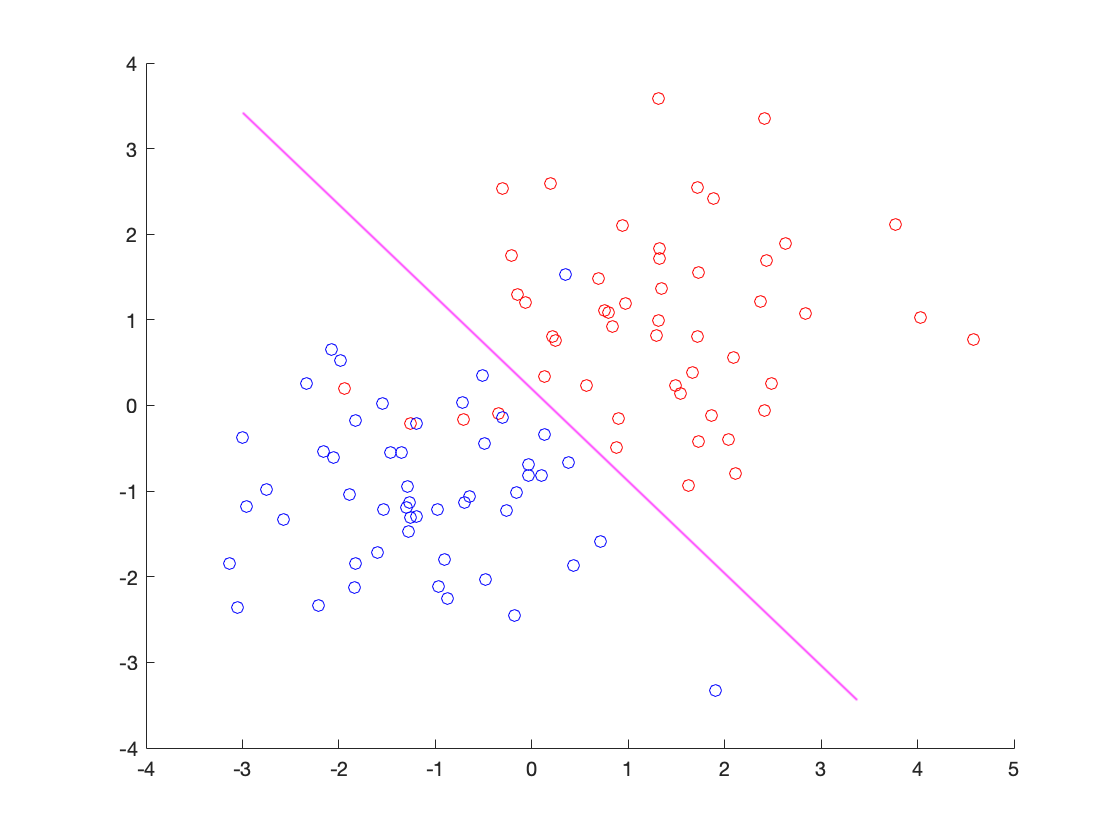
\includegraphics[width=8cm]{images/gaussians.png}
    \caption{Optimal decision boundary}
    \label{fig:gaussians}
\end{figure}

\subsection{Support vector machine classifier}

A support vector is the data point that is closest to the hyperplane. Therefore, a data point becomes a support vector when it is closer to the hyperplane. The data points that are closer to the hyperplane influence the hyperplane's orientation and position in the sense that potential modifications of a support vector's position will also affect the orientation and the position of the hyperplane. Their importance changes with regards to the hyperplane, since by removing or changing the position of a support vector, the position of the hyperplane also changes. This is illustrated in Figure \ref{fig:influence}, where we can see that the addition of extra support vectors changes the position and orientation of the hyperplane. 

\begin{figure*}[]
    \centering
    \begin{subfigure}{0.4\linewidth}
        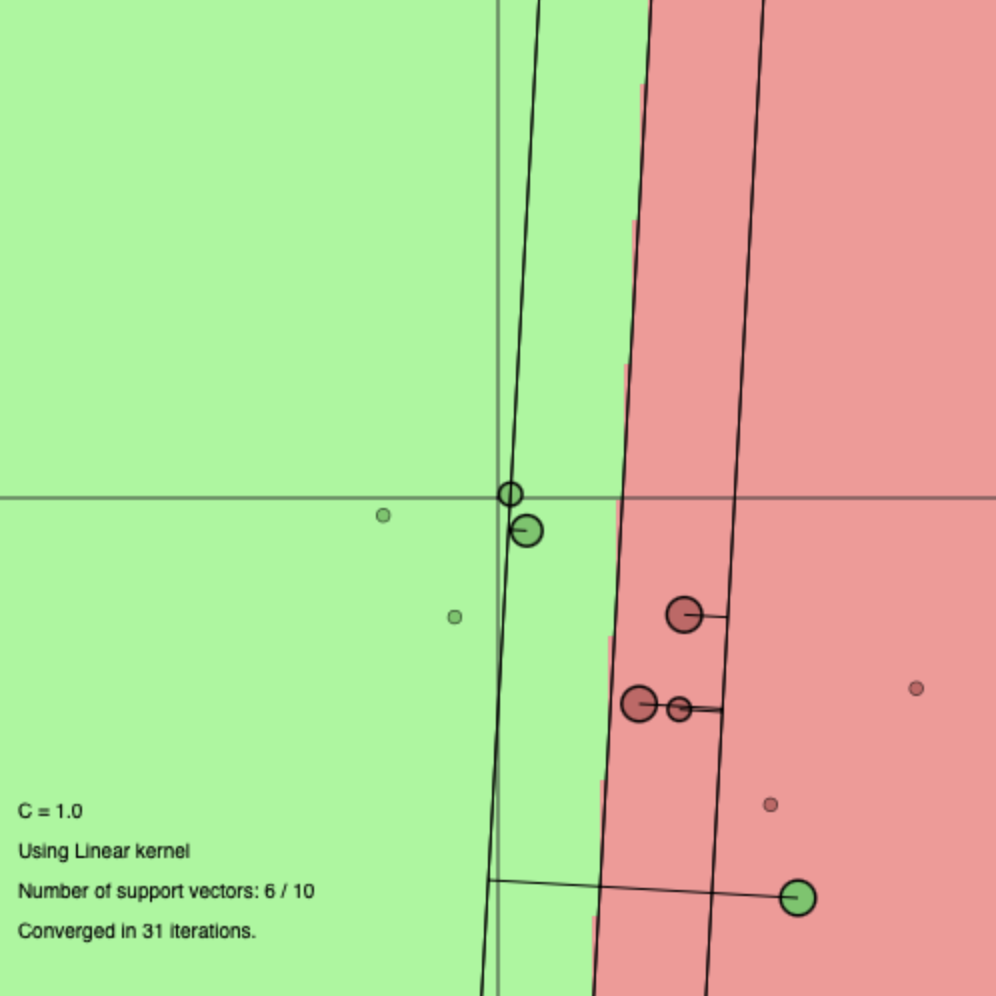
\includegraphics[width=\linewidth]{images/sup_imp_2.png}
        \caption{Initial}
    \end{subfigure}
    \begin{subfigure}{0.4\linewidth}
        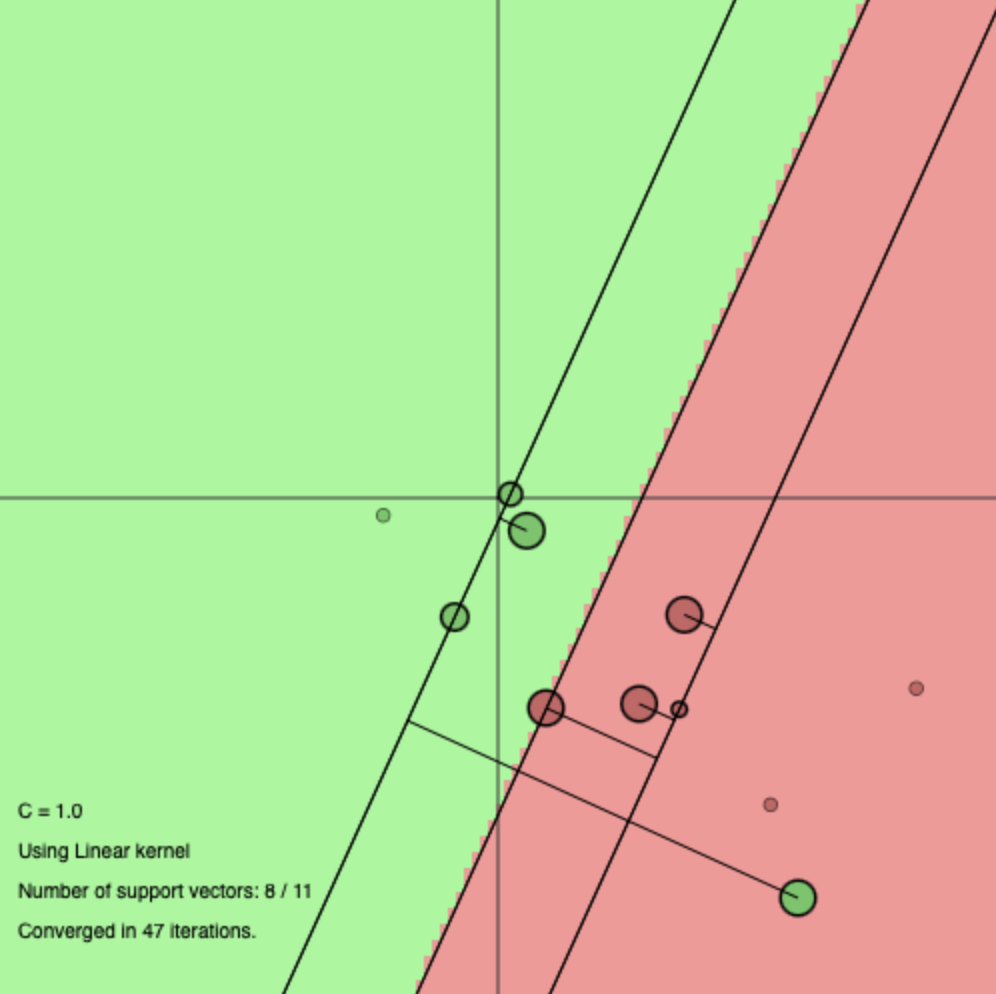
\includegraphics[width=\linewidth]{images/sup_imp_1.png}
        \caption{Addition of support vectors}
    \end{subfigure}
    \caption{Addition of new support vectors influence on the hyperplane}
    \label{fig:influence}
\end{figure*}

The addition of more datapoints to the dataset, when on the right side, do not greatly affect the outcome of the decision boundary, as opposed to additions on the wrong side, which have a significant effect. This happes due to the fact that additions on the wrong side increase the penalty applied for misclassification errors. This is illustrated in Figure \ref{fig:svm_addition_side}.

\begin{figure*}[]

        \begin{subfigure}{0.33\linewidth}
            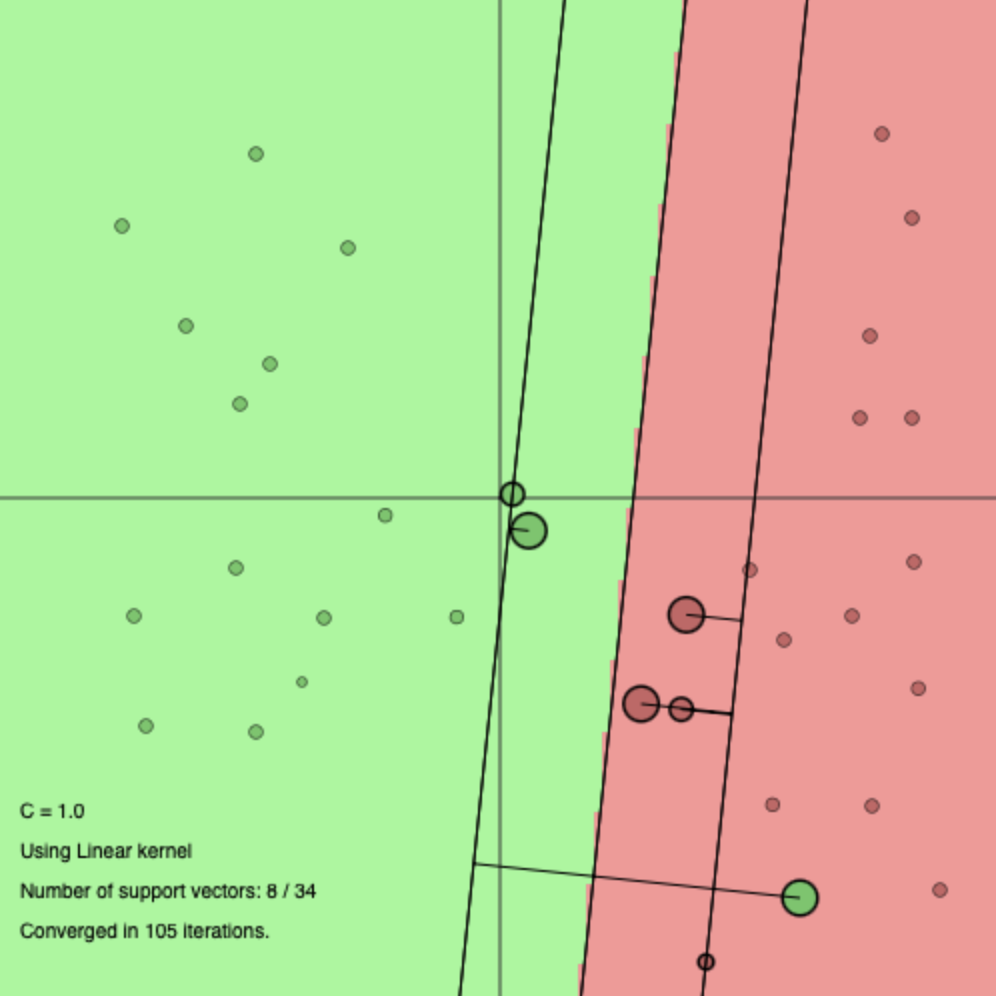
\includegraphics[width=\linewidth]{images/lin_initial.png}
            \caption{initial}
        \end{subfigure}
        \begin{subfigure}{0.33\linewidth}
            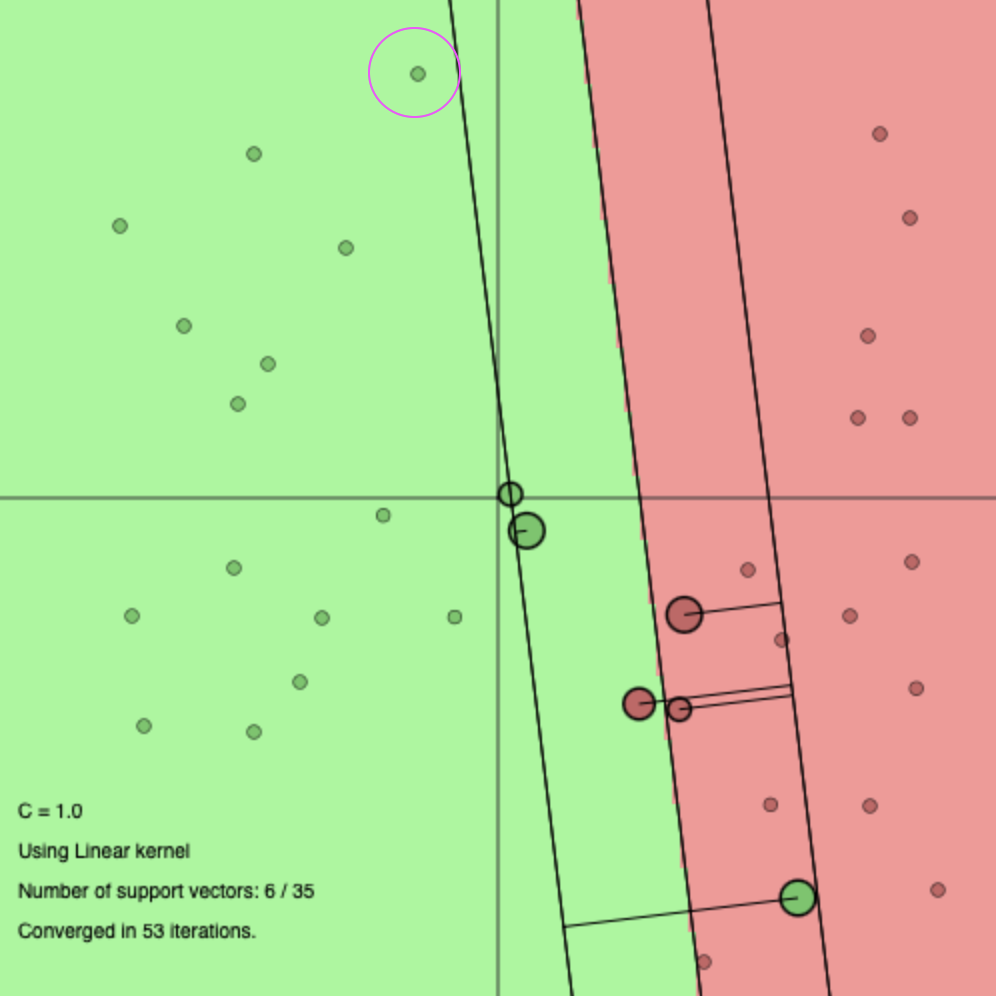
\includegraphics[width=\linewidth]{images/lin_right_green.png}
            \caption{Right side (green)}
        \end{subfigure}
        \begin{subfigure}{0.33\linewidth}
            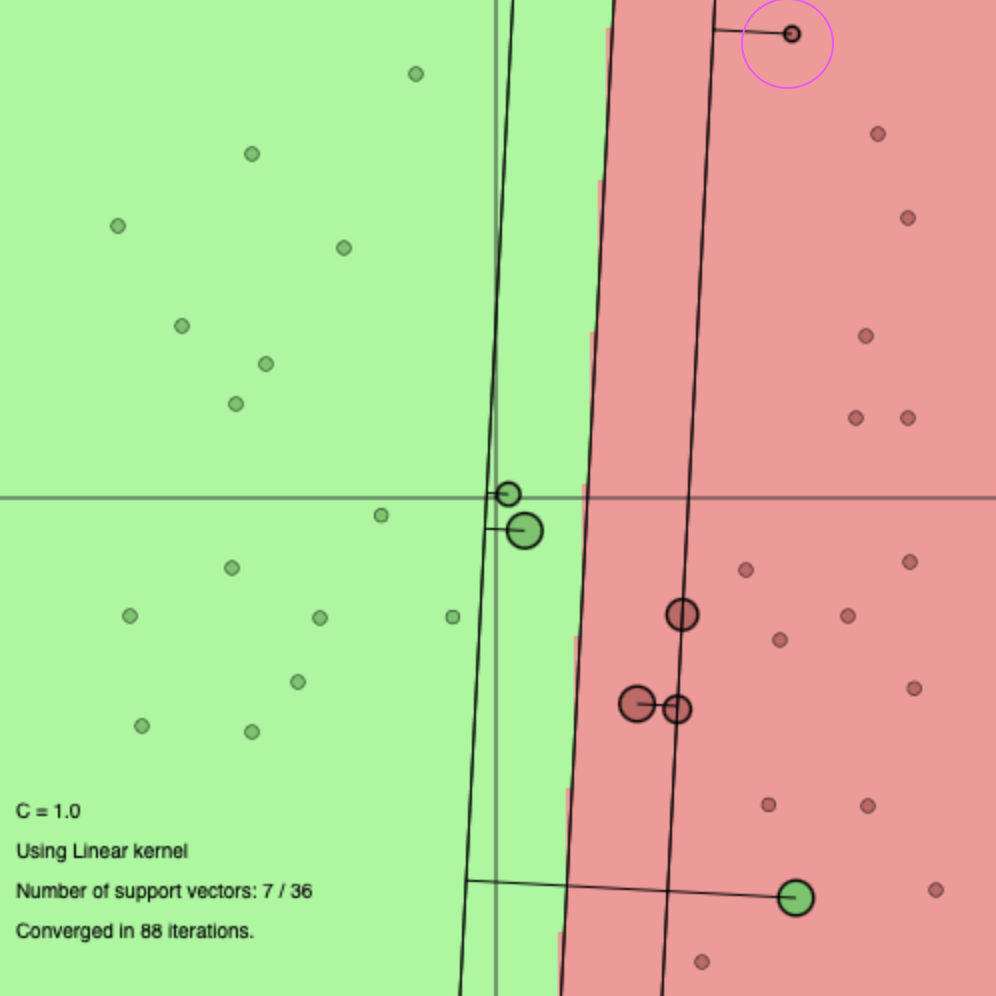
\includegraphics[width=\linewidth]{images/lin_right_red.png}
            \caption{Right side (red)}
        \end{subfigure}

		\begin{subfigure}{0.33\linewidth}
            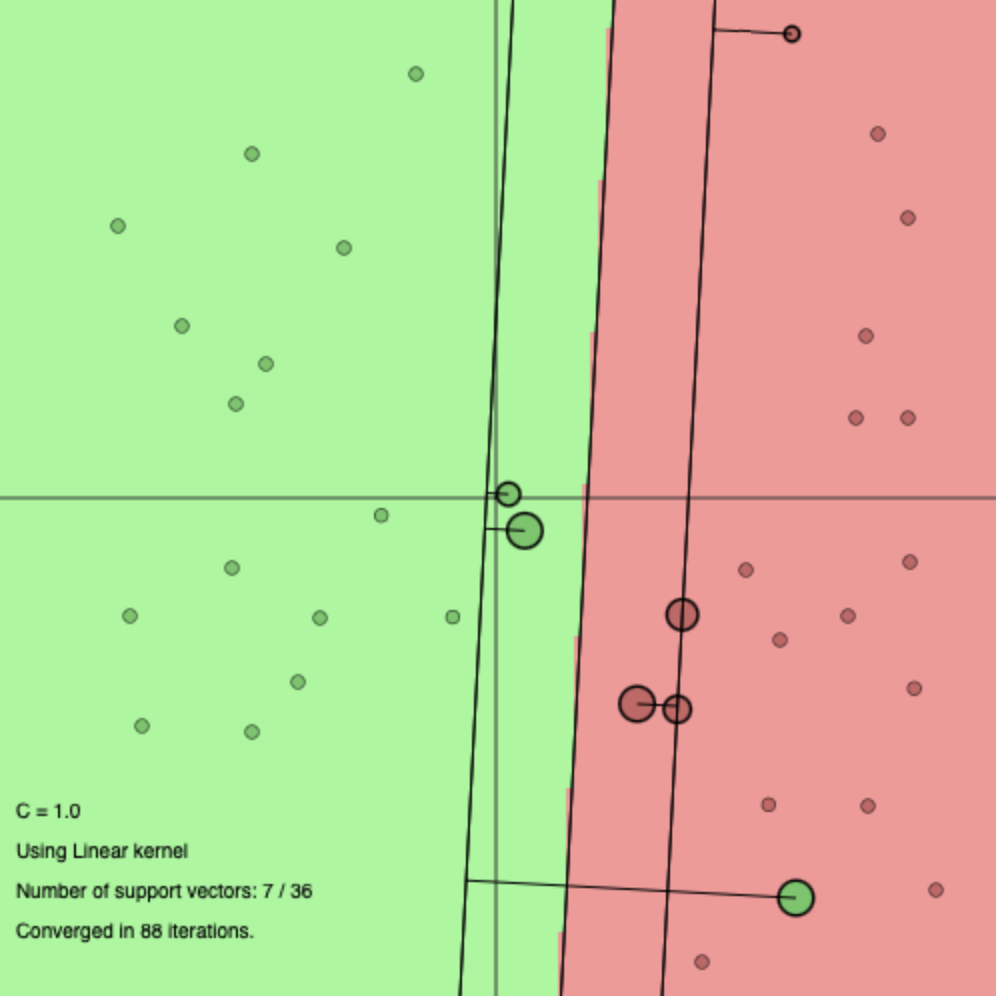
\includegraphics[width=\linewidth]{images/lin_right_red_2.png}
            \caption{initial}
        \end{subfigure}
        \begin{subfigure}{0.33\linewidth}
            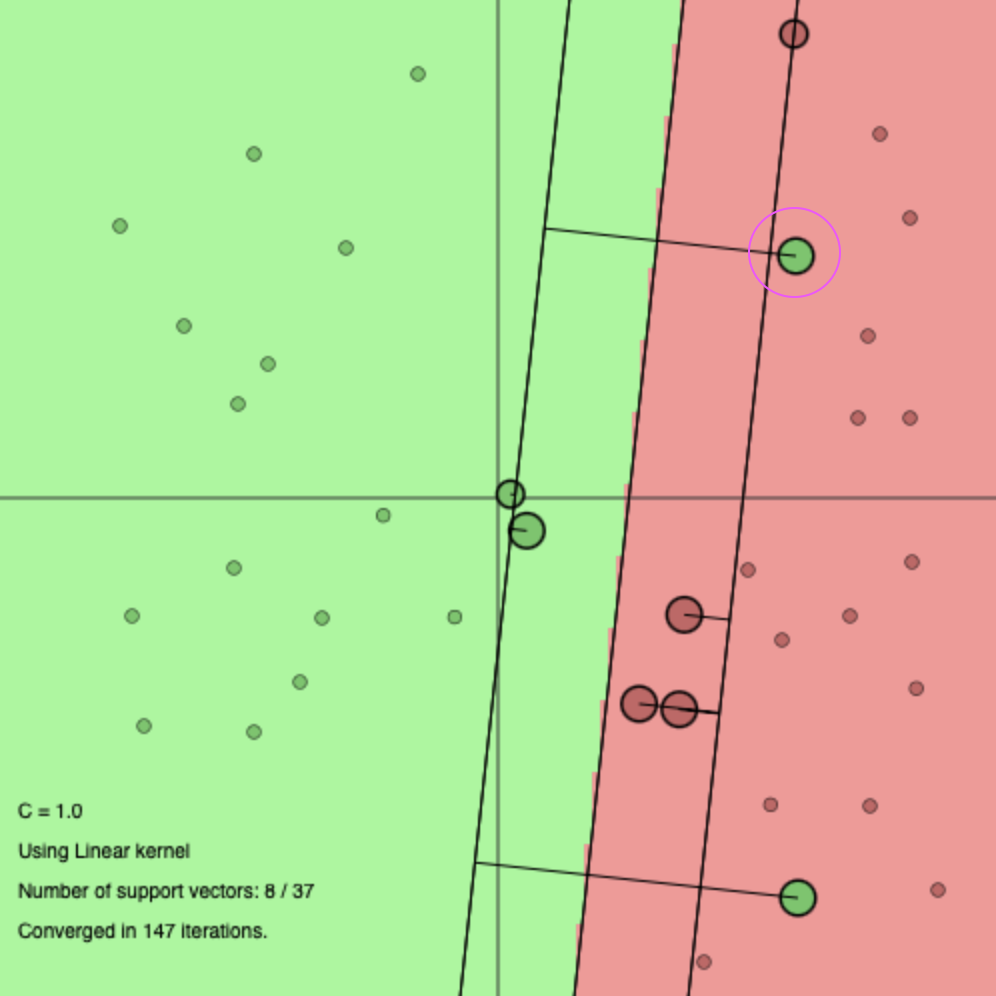
\includegraphics[width=\linewidth]{images/lin_wrong_green.png}
            \caption{Wrong side (green)}
        \end{subfigure}
        \begin{subfigure}{0.33\linewidth}
            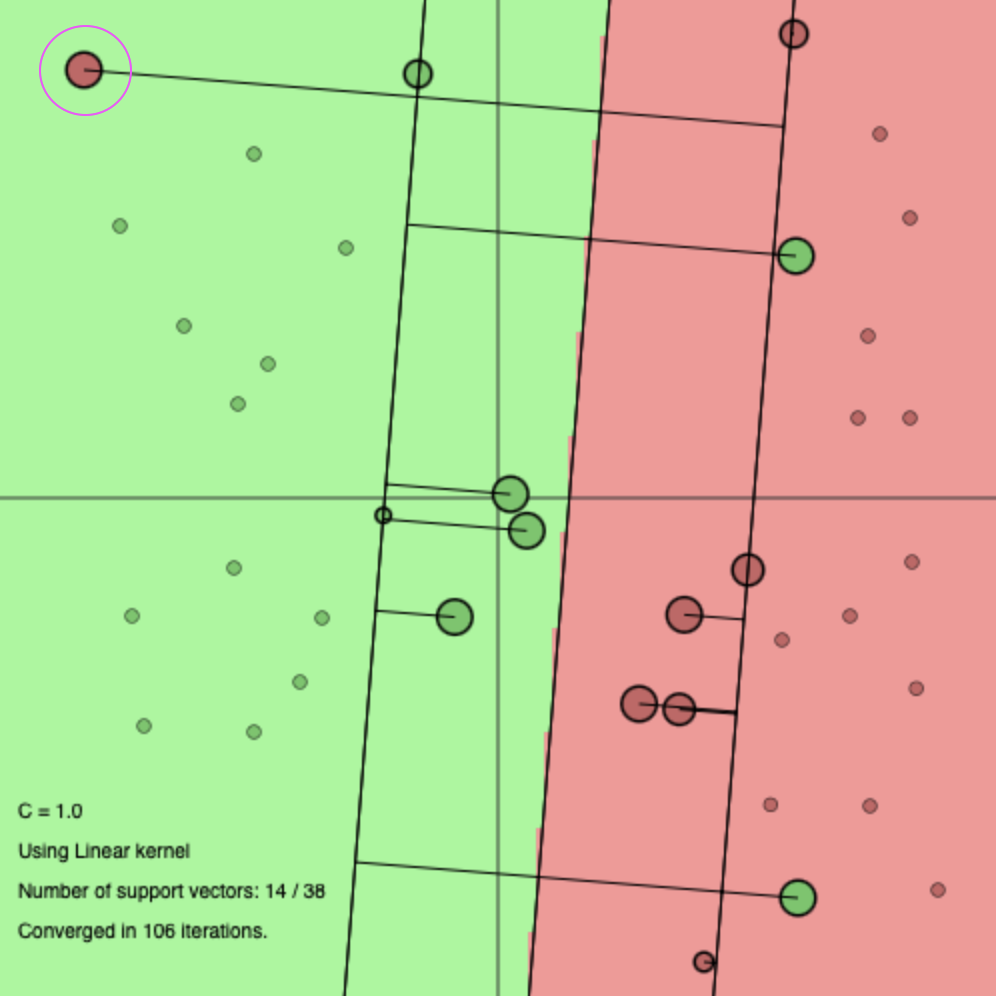
\includegraphics[width=\linewidth]{images/lin_wrong_red.png}
            \caption{Wrong side (red)}
        \end{subfigure}
  
        \caption{Illustration of the effect of the addition of new datapoints in the hyperplane}
        
        \label{fig:svm_addition_side}
\end{figure*}

The regularization hyperparameter $C$ is responsible for handling misclassification errors. For larger values of $C$ we observe that the hyperplane becomes more narrow, whereas for smaller ones it becomes less narrow. This is explained by the fact that the optimization will choose a hyperplane with a smaller margin that classifies all the training points correctly (for larger values of $C$). Conversely, significantly smaller values lead to larger margins in the hyperplane, even though the hyperplane misclassifies more points. This is illustrated in Figure \ref{fig:linear_c}.

The parameter $\sigma$ is the radius that determines the influence that a single training example has on the classification . Specifically, when the distance from a datapoint exceeds $\sigma$, the datapoints will become too similar, which can lead to underfitting. In contrast, for very small values of $\sigma$ the examples become too dissimilar, thus leading to overfitting. This is depicted in Figure \ref{fig:c_and_sigma}. 

\begin{figure*}[]
    \begin{subfigure}{0.33\linewidth}
        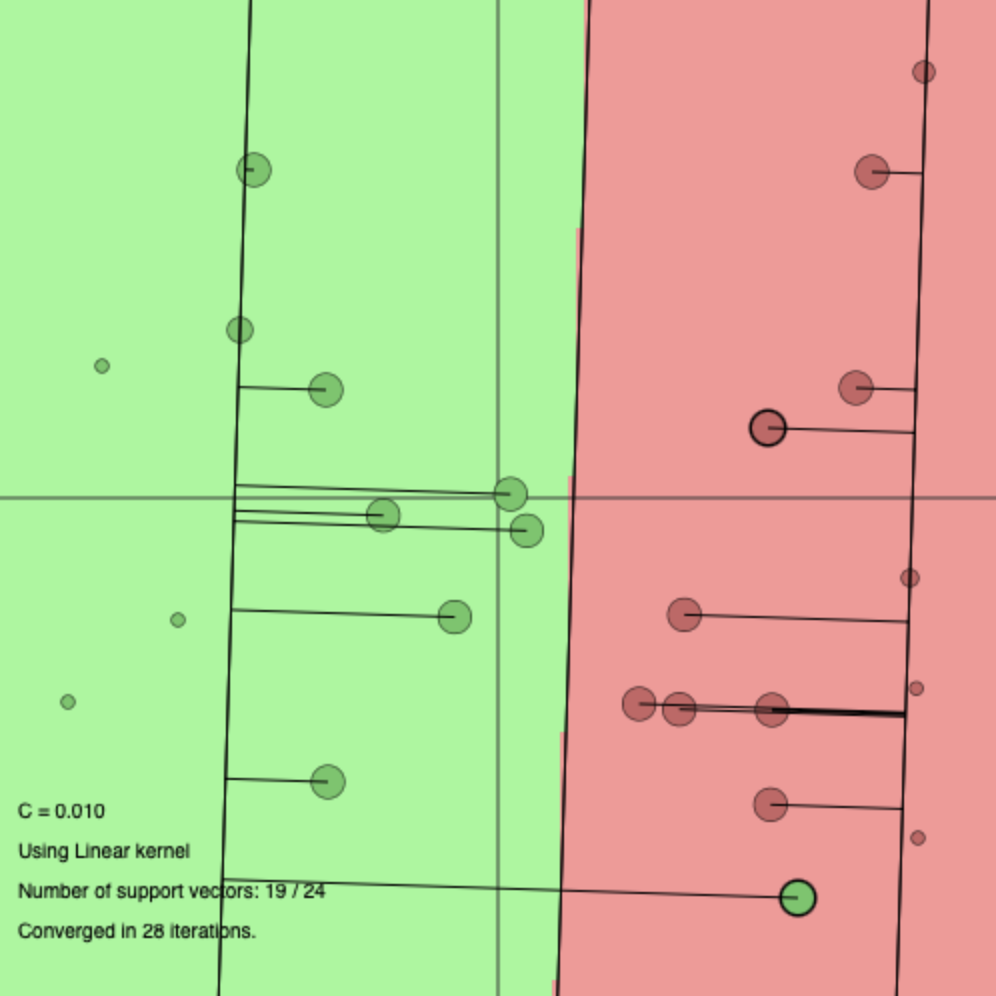
\includegraphics[width=\linewidth]{images/lin_c_001.png}
        \caption{c=0.01}
    \end{subfigure}
    \begin{subfigure}{0.33\linewidth}
        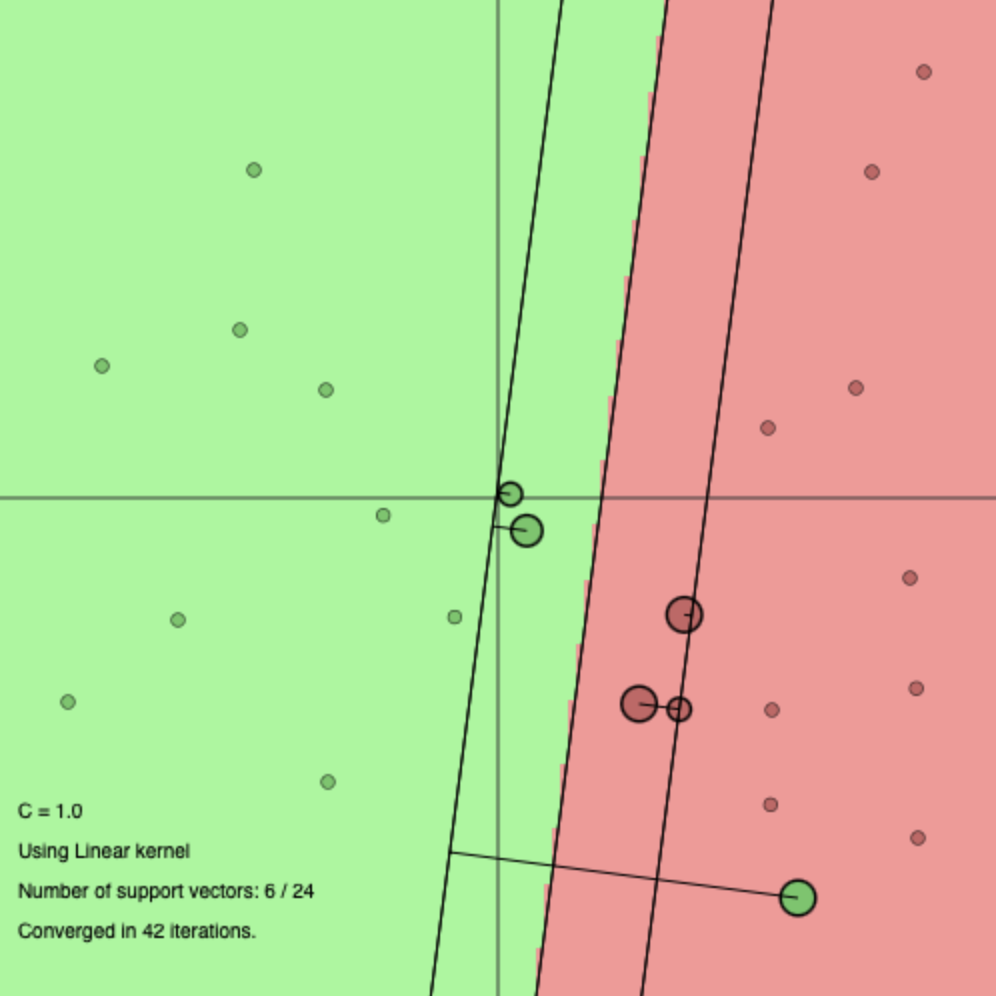
\includegraphics[width=\linewidth]{images/lin_c_1.png}
        \caption{c=1}
    \end{subfigure}
    \begin{subfigure}{0.33\linewidth}
        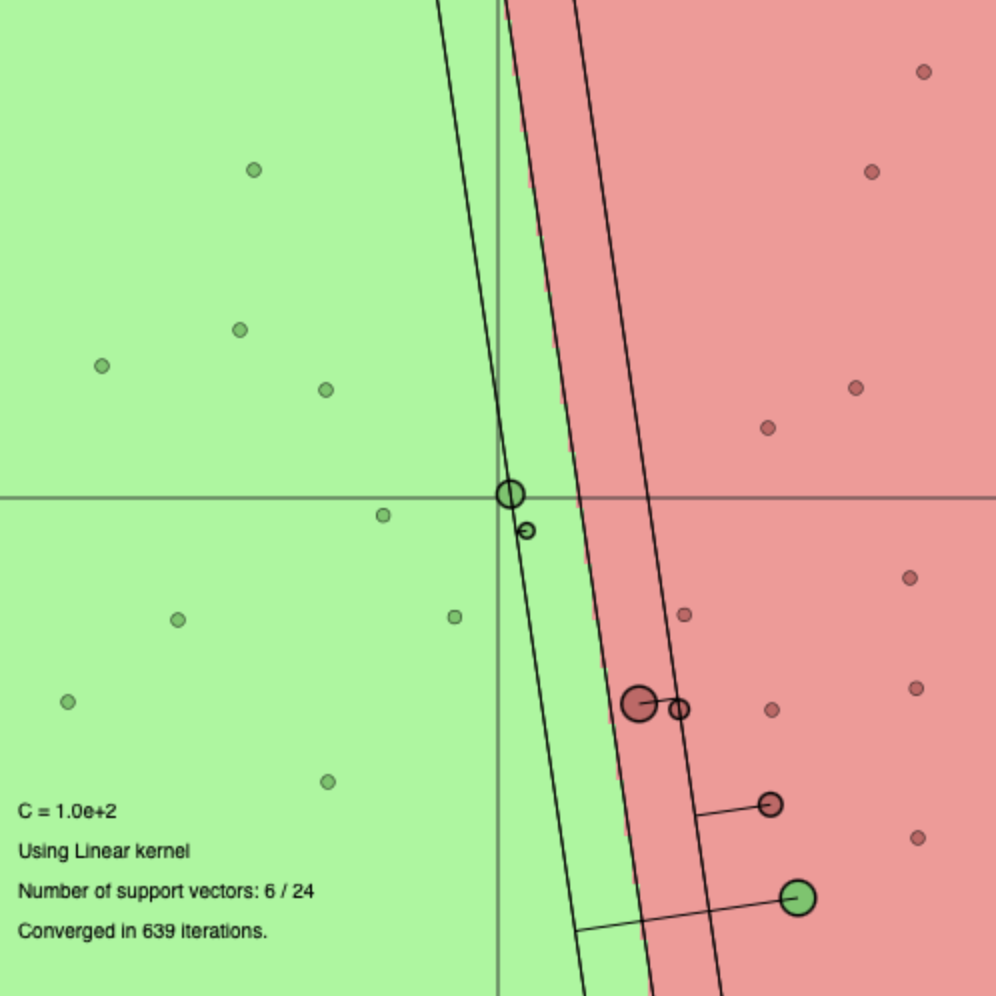
\includegraphics[width=\linewidth]{images/lin_c_100.png}
        \caption{c=100}
    \end{subfigure}
    \caption{Various values for hyperparameter c in linear kernel}
    \label{fig:linear_c}
\end{figure*}

\begin{figure*}
\begin{subfigure}{0.3\textwidth}
   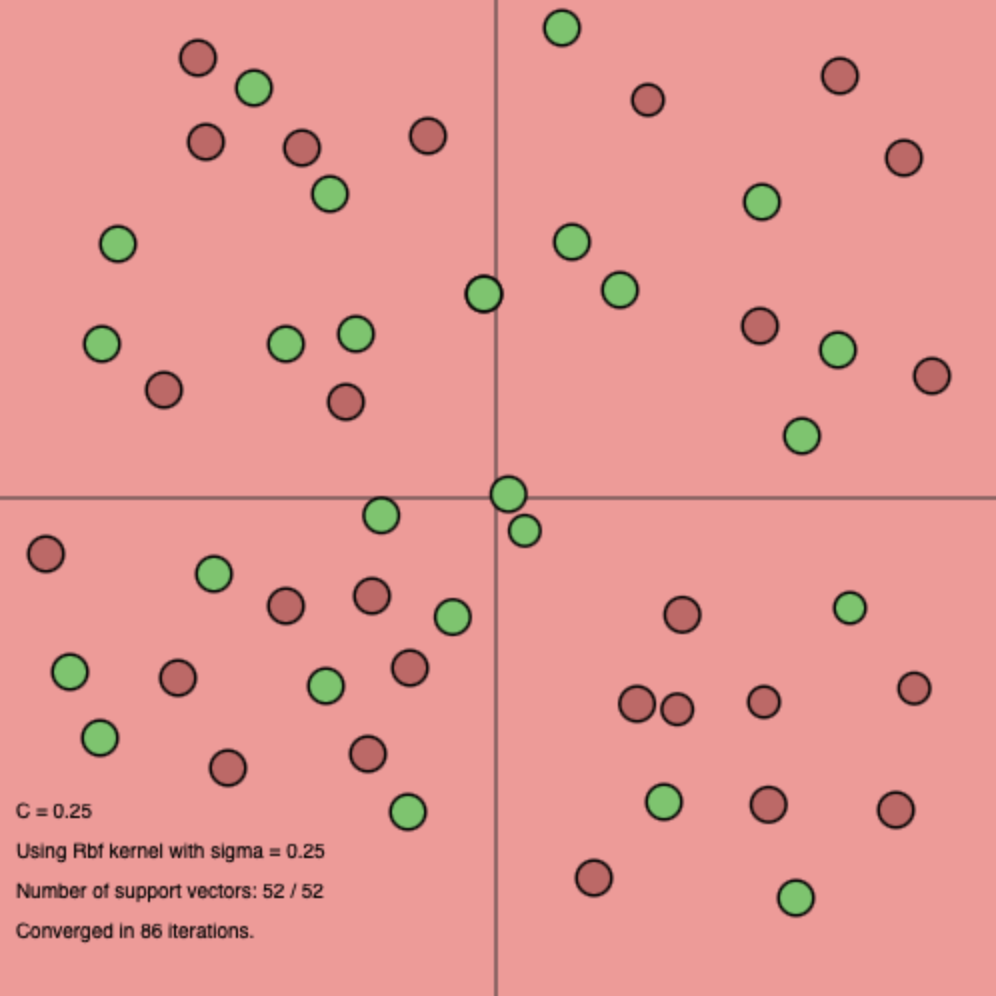
\includegraphics[width=\linewidth]{images/rbf_c_0.25_s_0.25.png}
   \caption{$c=0.25$, $\sigma=0.25$} \label{fig:x_a}
\end{subfigure}
\hspace*{\fill}
\begin{subfigure}{0.3\textwidth}
   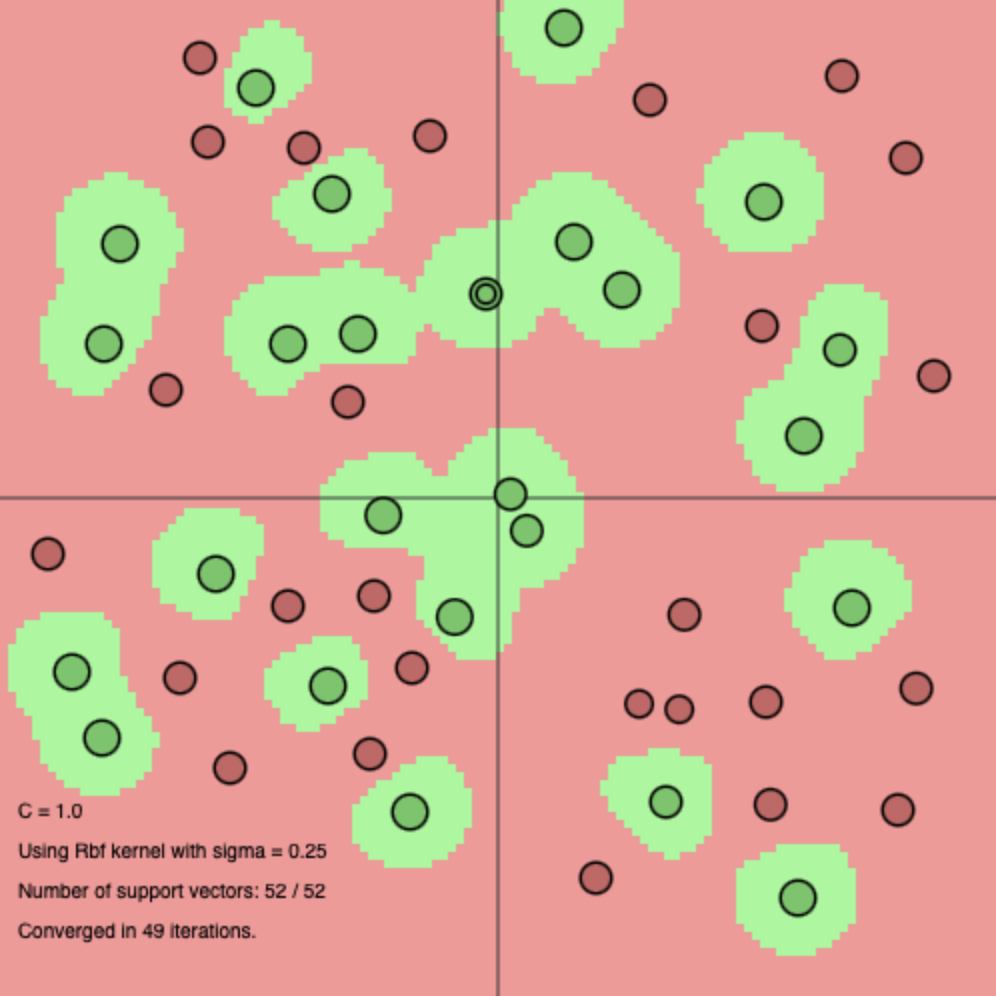
\includegraphics[width=\linewidth]{images/rbf_c_1_s_0.25.png}
   \caption{$c=1$, $\sigma=0.25$} \label{fig:x_b}
\end{subfigure}
\hspace*{\fill}
\begin{subfigure}{0.3\textwidth}
   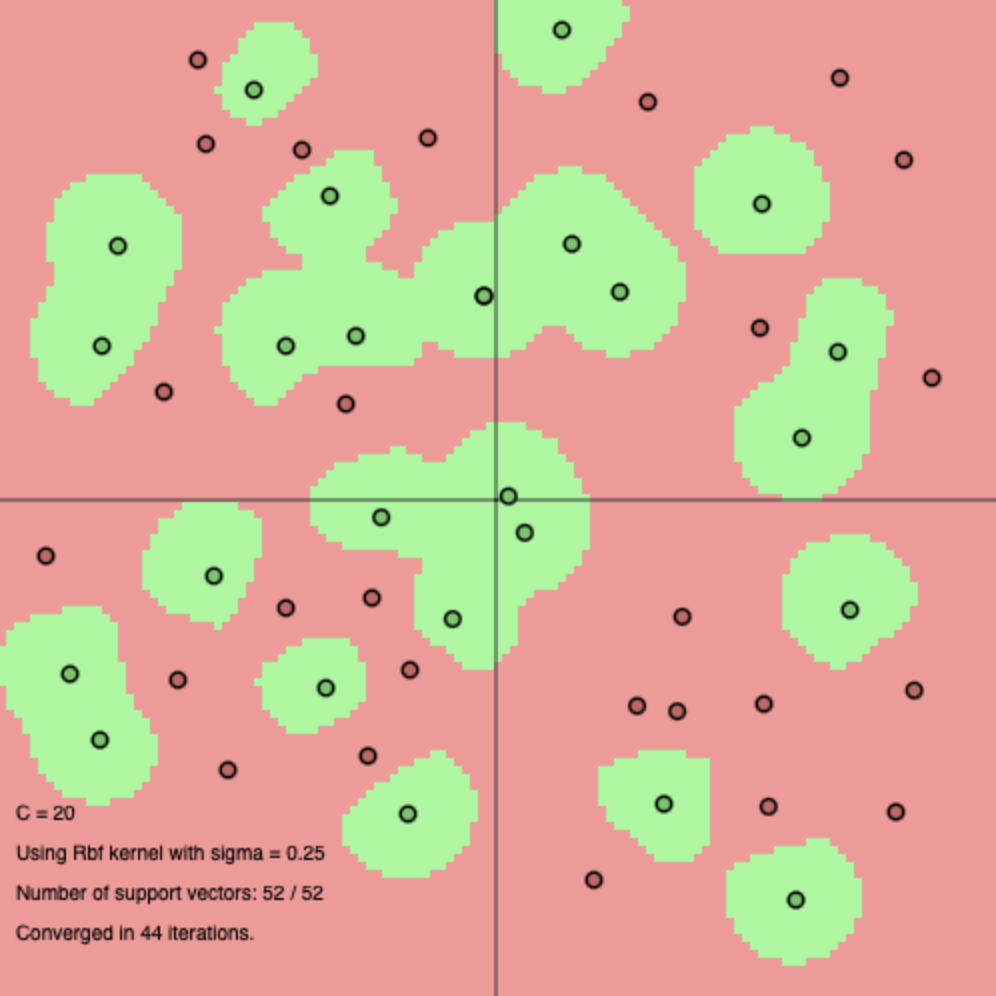
\includegraphics[width=\linewidth]{images/rbf_c_20_s_0.25.png}
   \caption{$c=20$, $\sigma=0.25$} \label{fig:x_c}
\end{subfigure}

\bigskip
\begin{subfigure}{0.3\textwidth}
   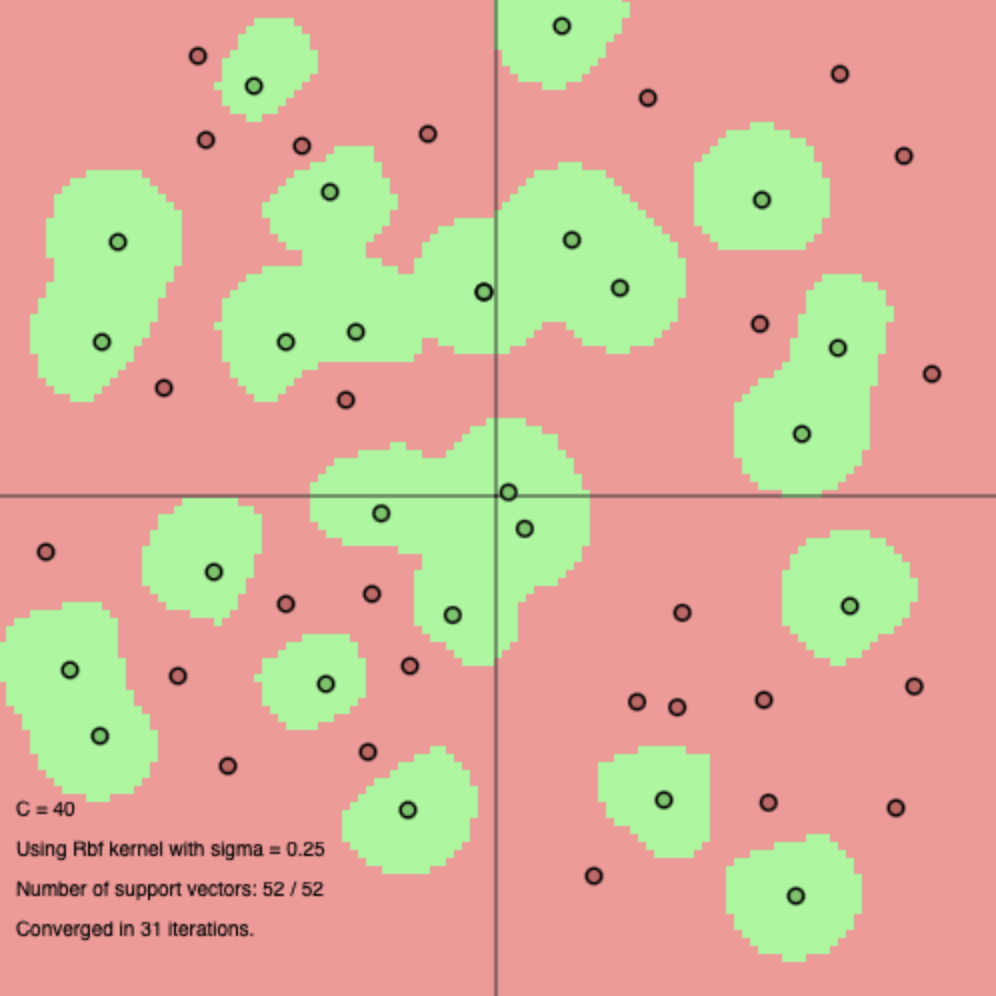
\includegraphics[width=\linewidth]{images/rbf_c_40_s_0.25.png}
   \caption{$c=40$, $\sigma=0.25$} \label{fig:x_d}
\end{subfigure}
\hspace*{\fill}
\begin{subfigure}{0.3\textwidth}
   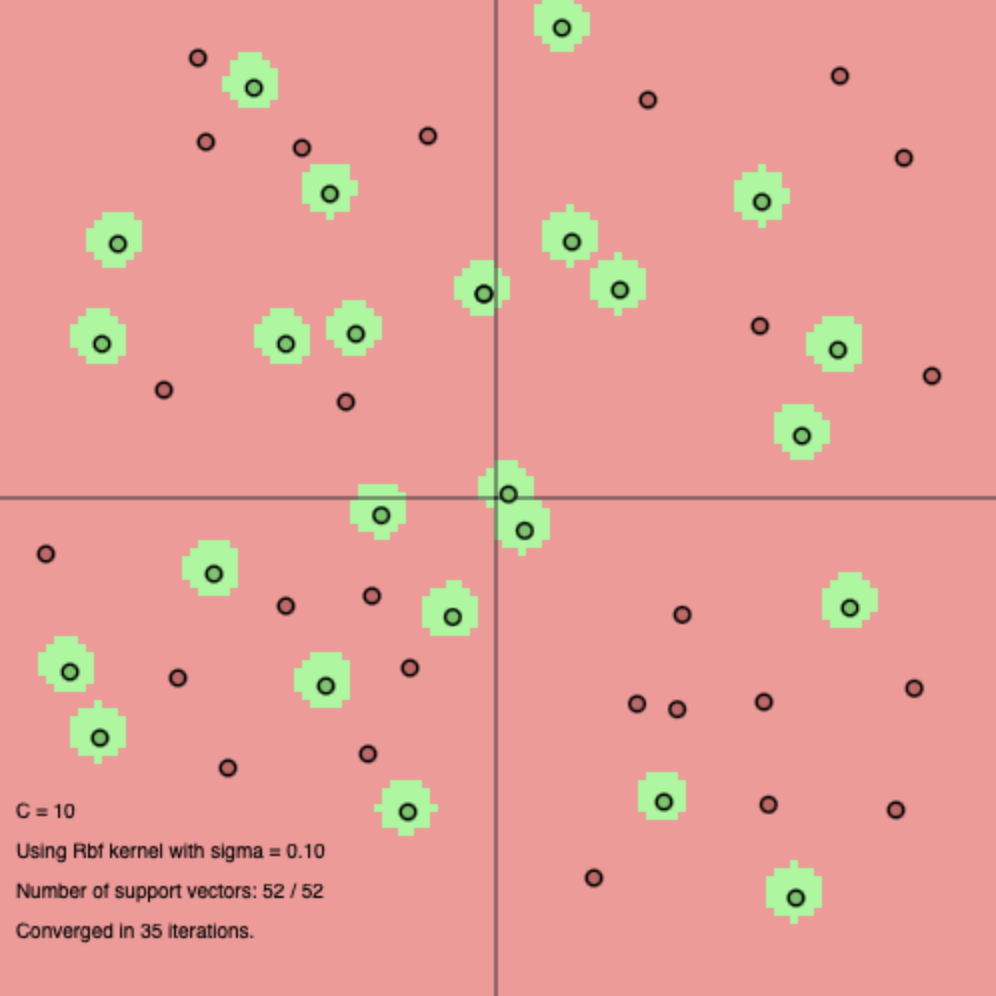
\includegraphics[width=\linewidth]{images/rbf_c_10_s_0.1.png}
   \caption{$c=10$, $\sigma=0.1$} \label{fig:x_e}
\end{subfigure}
\hspace*{\fill}
\begin{subfigure}{0.3\textwidth}
   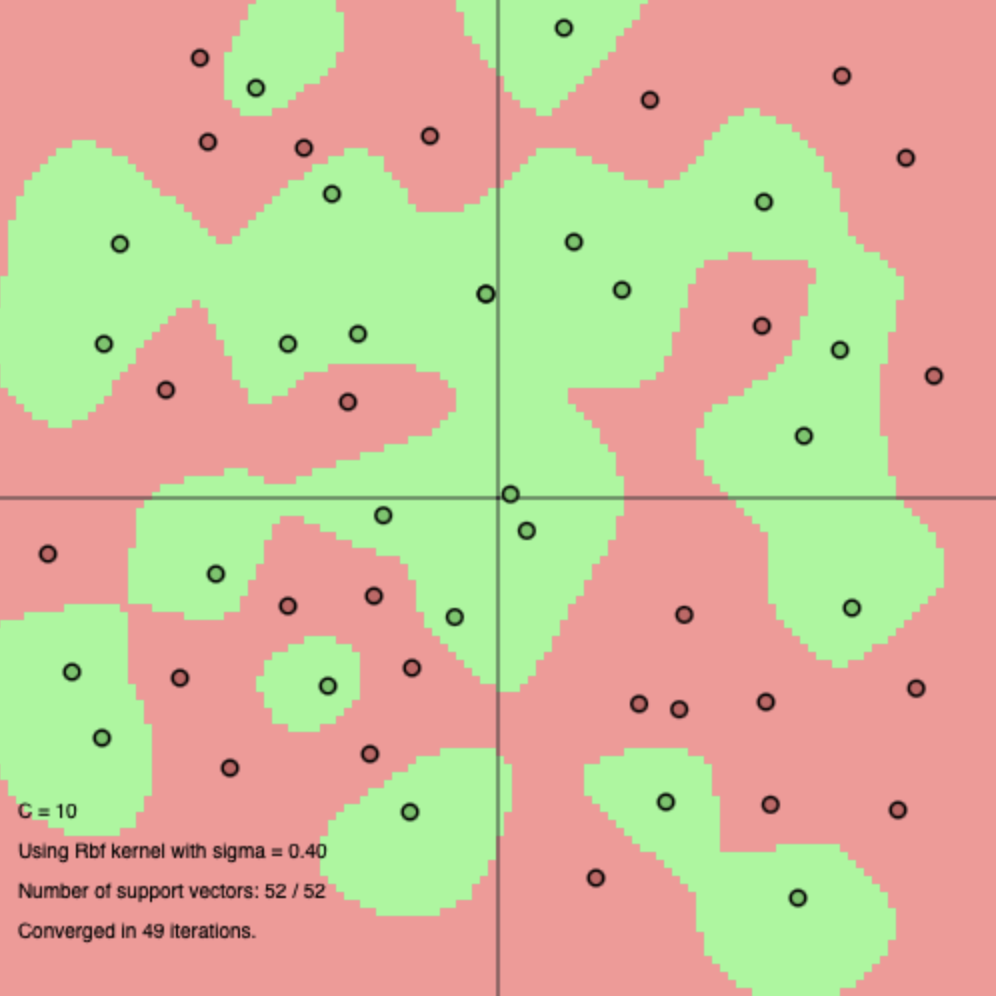
\includegraphics[width=\linewidth]{images/rbf_c_10_s_0.4.png}
   \caption{$c=10$, $\sigma=0.4$} \label{fig:x_f}
\end{subfigure}

\bigskip
\hspace*{\fill}
\begin{subfigure}{0.3\textwidth}
   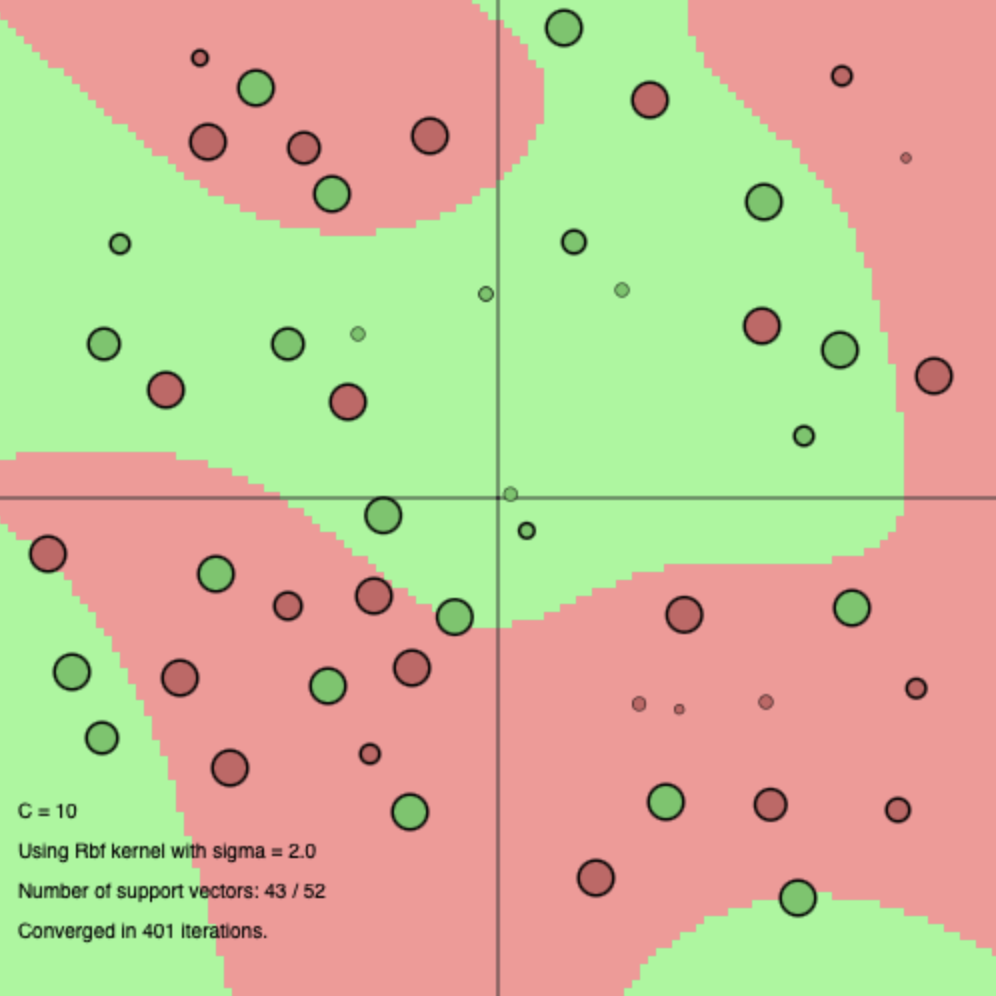
\includegraphics[width=\linewidth]{images/rbf_c_10_s_2.png}
   \caption{$c=10$, $\sigma=2$} \label{fig:x_g}
\end{subfigure}%
\hspace*{0.05\textwidth}%
\begin{subfigure}{0.3\textwidth}
   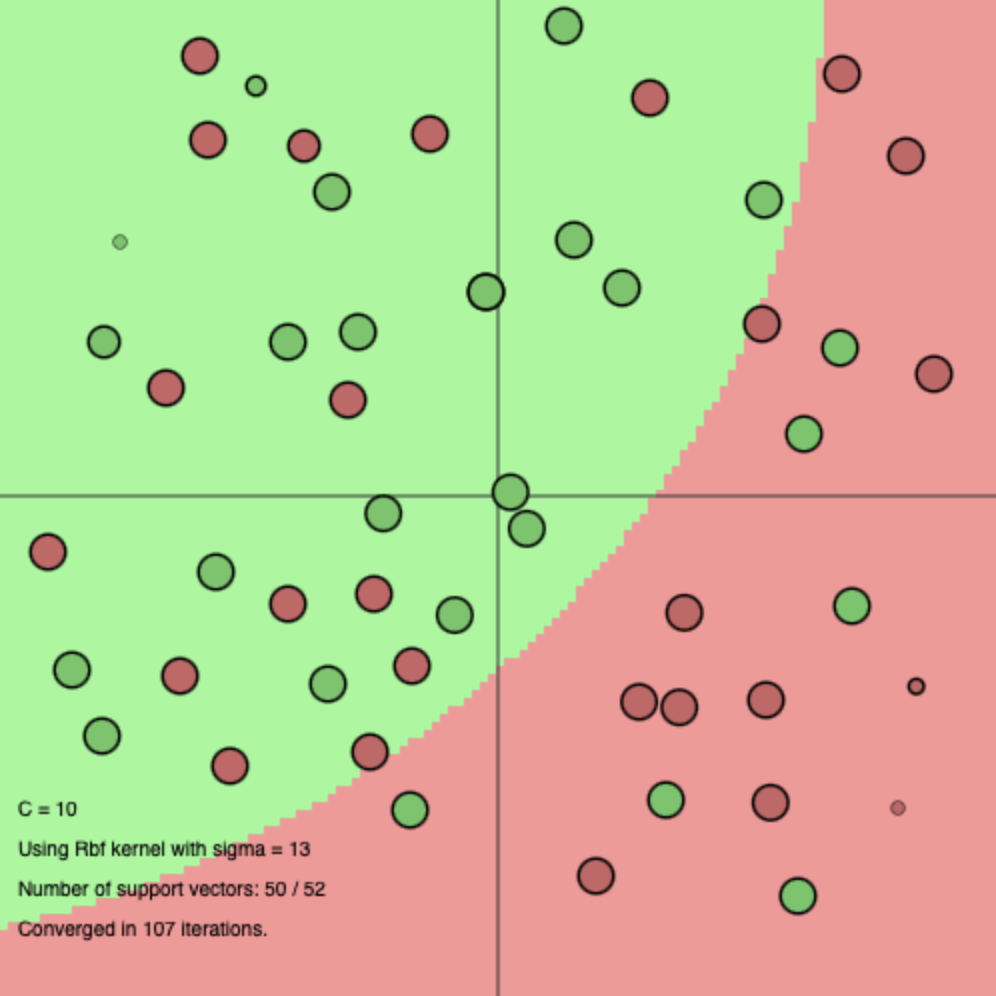
\includegraphics[width=\linewidth]{images/rbf_c_10_s_13.png}
   \caption{$c=10$, $\sigma=13$} \label{fig:x_h}
\end{subfigure}
\hspace*{\fill}

\caption{Various values for $c$ and $\sigma$ in the RBF kernel}
    \label{fig:c_and_sigma}
\end{figure*}

As we can see in Figure \ref{fig:lin_RBF_comparison} the Gaussian (RBF) kernel performs better than the linear kernel in our classification task. This is due to the fact that it can produce decision boundaries that are non-linear, in contrast to the linear kernel. The result of this is that the Gaussian kernel is able to capture more complex relationships among the datapoints. 

\begin{figure*}[]
    \centering
    \begin{subfigure}{0.4\linewidth}
        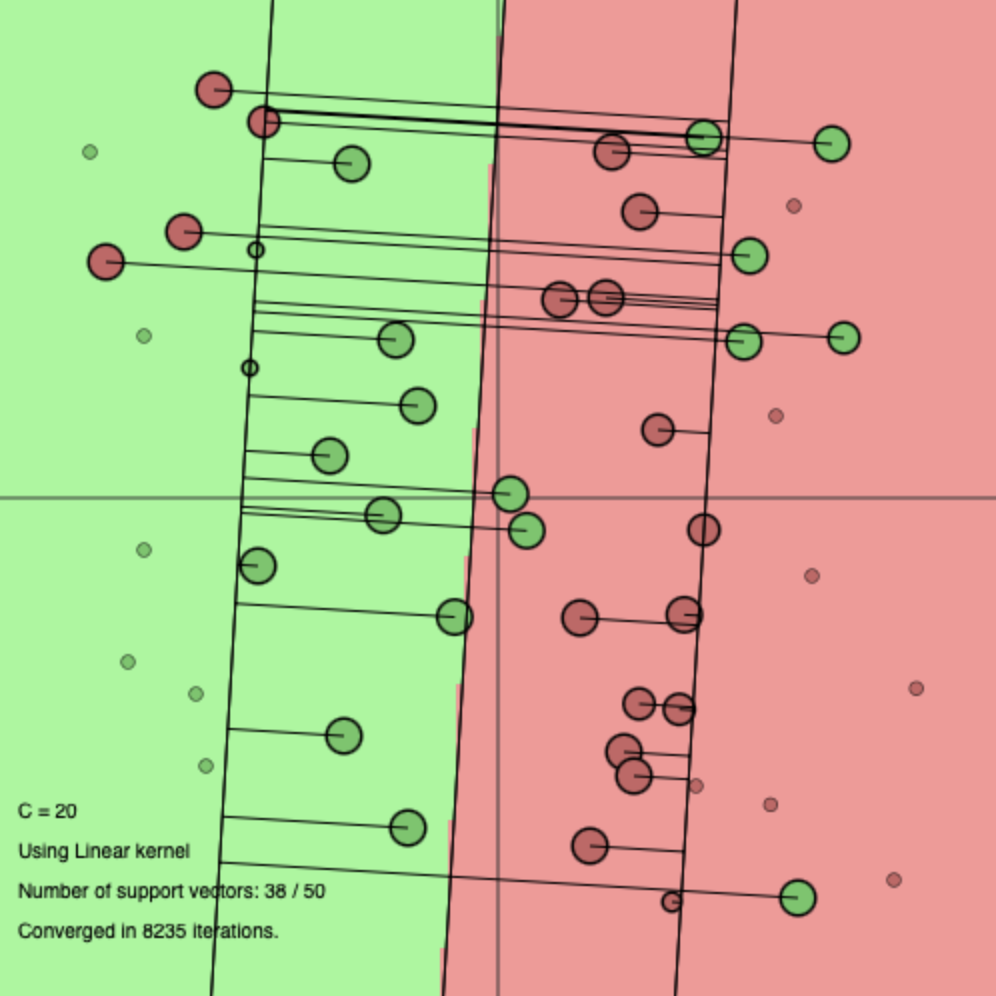
\includegraphics[width=\linewidth]{images/lin_comp.png}
        \caption{linear kernel}
    \end{subfigure}
    \begin{subfigure}{0.4\linewidth}
        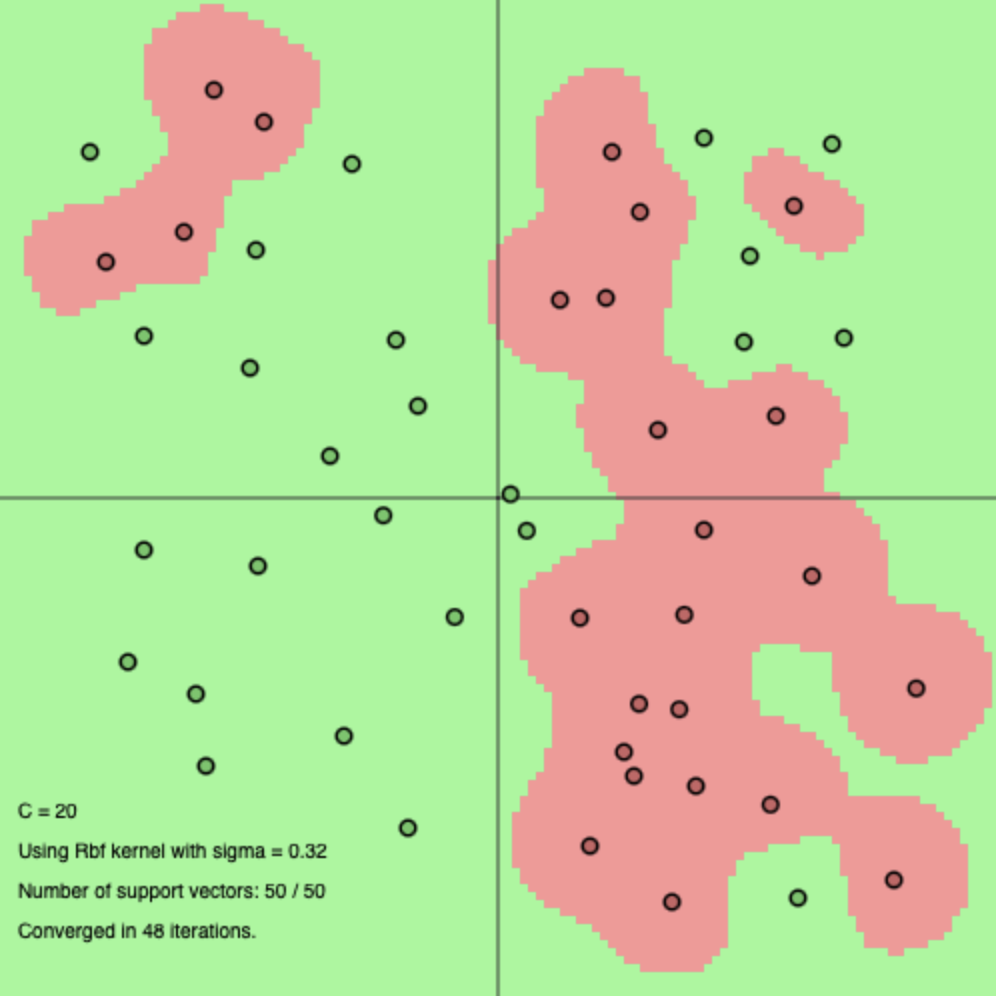
\includegraphics[width=\linewidth]{images/rbf_comp.png}
        \caption{RBF kernel}
    \end{subfigure}
    \caption{Comparison between linear and RBF kernel}
    \label{fig:lin_RBF_comparison}
\end{figure*}

\subsection{Least-squares support vector machine classifier}
\subsubsection{Influence of hyperparameters and kernel parameters}
In this section, the objective is to perform classification in the Iris dataset, by using the least squares based variant of the SVM (LS-SVM). Additionally, we want to experiment with different kernel functions and hyperparameters and investigate the effect they have on our classifier. Two different kernel functions were implemented; \textbf{polynomial kernel} and \textbf{RBF kernel}.

\textbf{Polynomial kernel} For polynomials with degree $d$, the polynomial kernel is defined as: 

\begin{equation}
K(x,x_k) = (x^Tx_k +\tau)^d
\end{equation} 
where $d$ corresponds to the degree of the polynomial kernel. The degree has a significant influence on the the decision boundary since it controls its flexibility. Higher degrees provide a more flexible decision boundary but at the same time increase the chance of overfitting. 

\textbf{RBF kernel}
RBF kernels are in general the most widely used kernels. For two datapoints $X1$ and $X2$, the RBF kernel function computes their similarity and is defined as:

\begin{equation}
K(X1,X2) = exp(-\frac{||X1-X2||^2_2}{\sigma^2})
\end{equation}
where $\sigma$ is the variance and $||X1-X2||$ is the Euclidean distance between two points $X1$ and $X2$.

In practice, the first choice in our experiments is a linear kernel, which is then followed by polynomial and RBF kernels, which improve the classification. In Figure \ref{fig:linpoly}, we can see the decision boundary for a linear kernel (a). Then, from (b) to (f) we can see the decision boundaries for polynomial kernels with varying degrees. As illustrated, a linear kernel has a high classification error of $55\%$ ($11$ out of $20$ examples misclassified). For the remaining polynomial kernels, we can see a significant improvement in degrees $2$ to $4$ where the classification error drops to $5\%$ and then to $0\%$. Finally, as the degree increases (higher than $15$), the classification error increases as well. This is visualized in (h) and (i). In Figure \ref{fig:rbfvarcsigma} we can see the effects of varying $\gamma$ and $\sigma^2$, which was discussed in the previous section. After the experiments, it was observed that the best results were obtained with a $\sigma^2$ in the range of $0.05$ to $15$ and for $\gamma$ between $0.5$ to $50$. 

\begin{figure*}[]

        \begin{subfigure}{0.33\linewidth}
            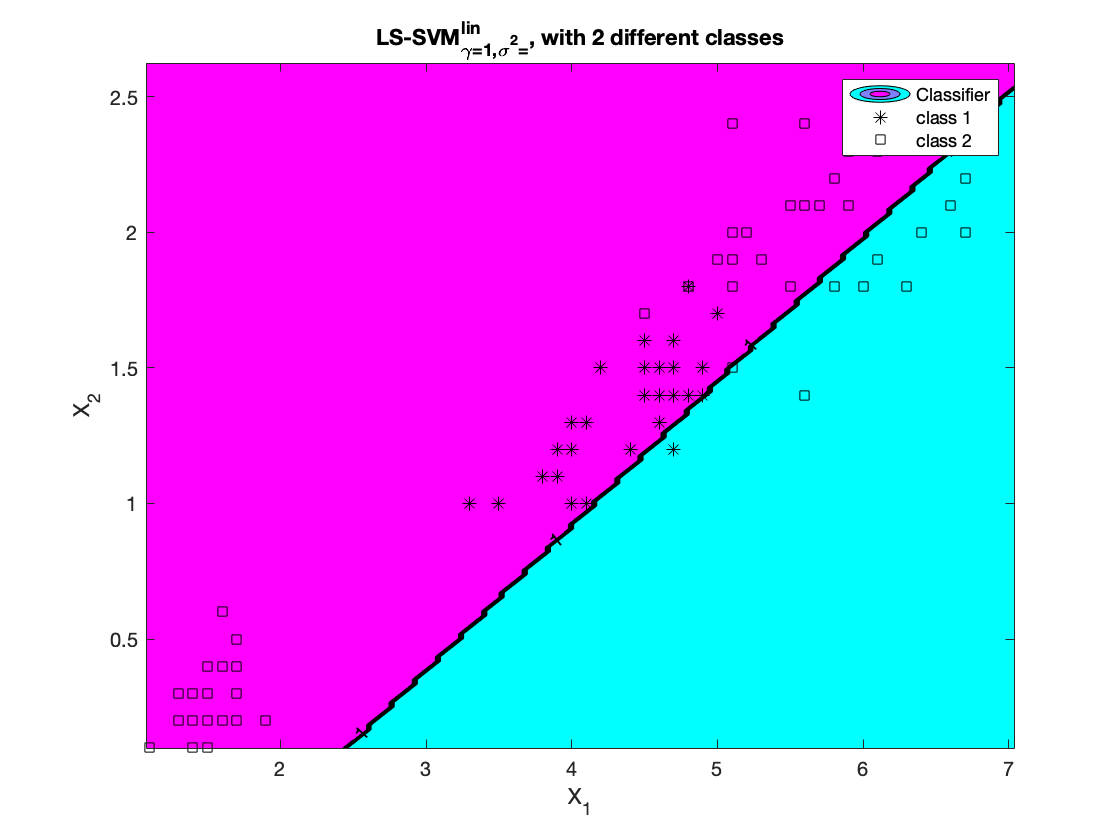
\includegraphics[width=\linewidth]{images/lssvm_lin.png}
            \caption{linear}
        \end{subfigure}
        \begin{subfigure}{0.33\linewidth}
            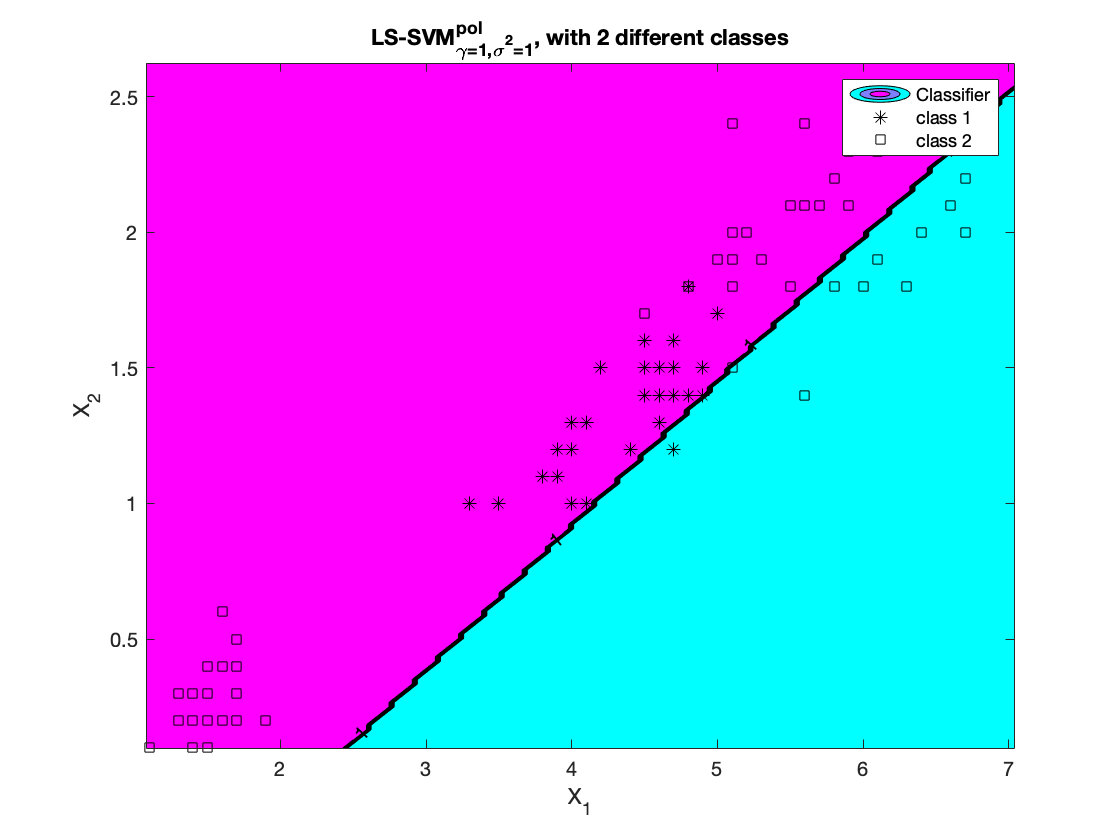
\includegraphics[width=\linewidth]{images/lssvm_poly_deg1.png}
            \caption{d = 1}
        \end{subfigure}
        \begin{subfigure}{0.33\linewidth}
            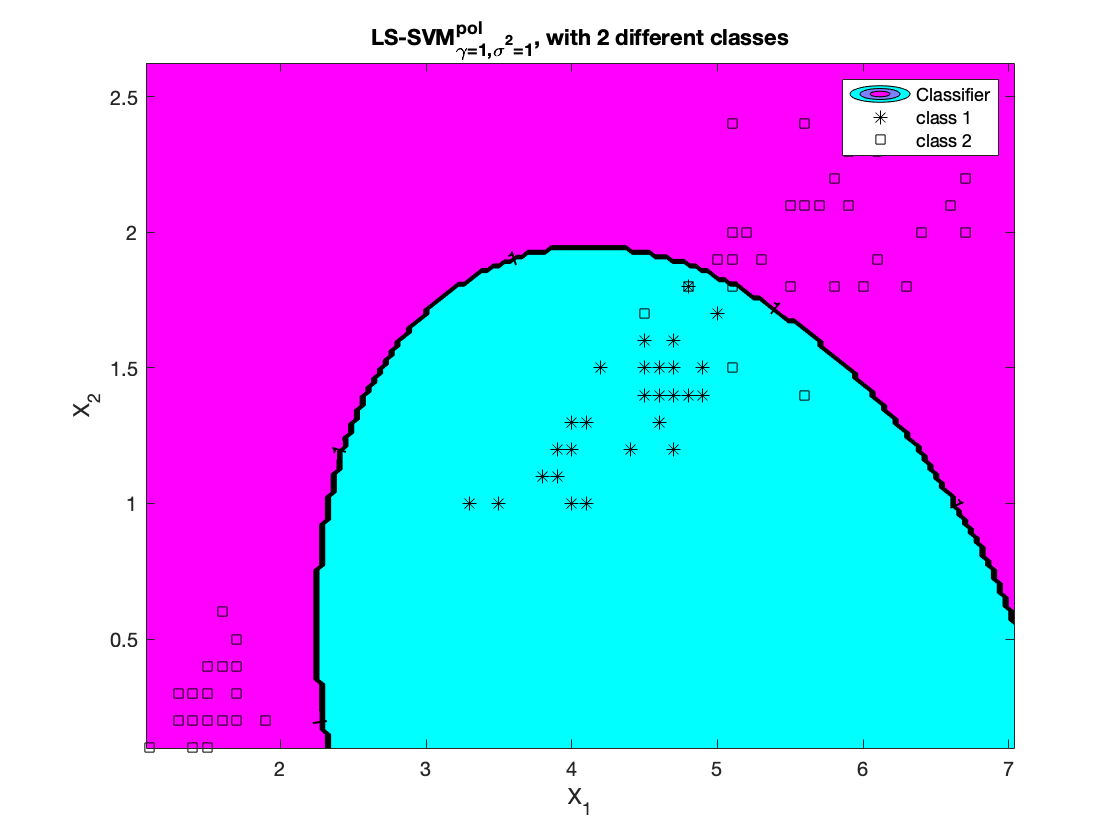
\includegraphics[width=\linewidth]{images/ls_svm_poly_deg2.png}
            \caption{d = 2}
        \end{subfigure}

		\begin{subfigure}{0.33\linewidth}
            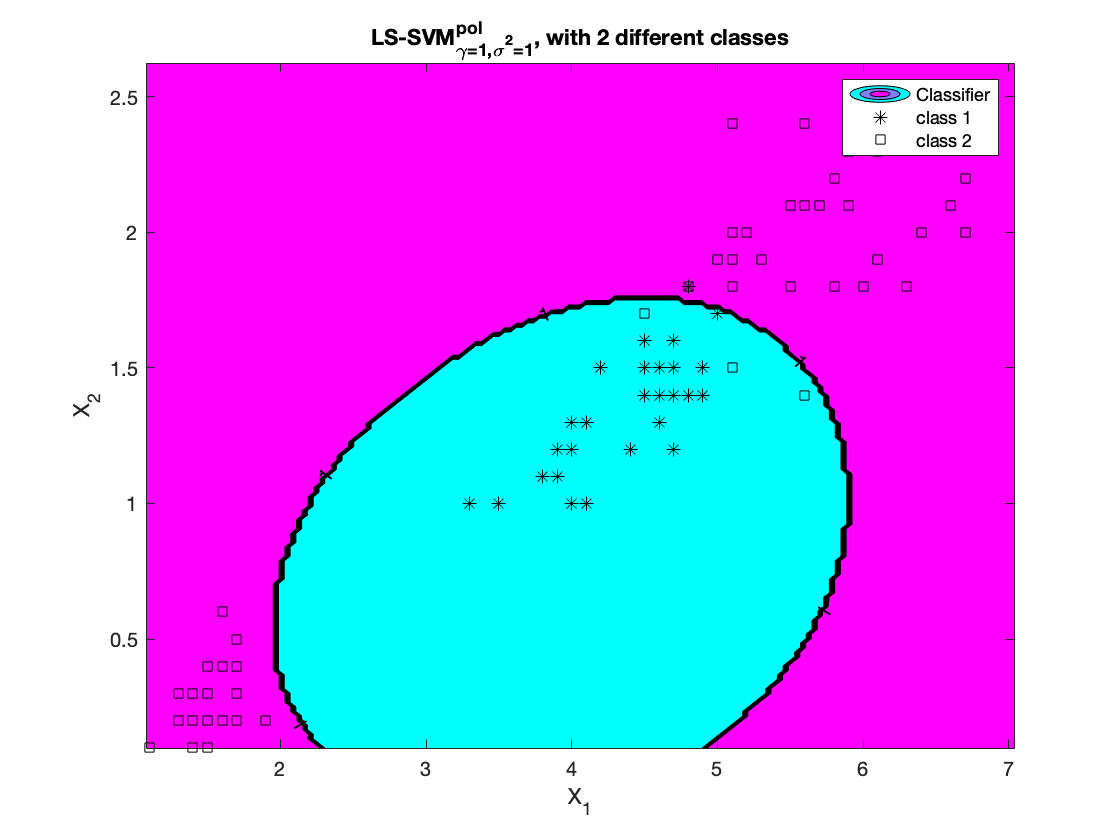
\includegraphics[width=\linewidth]{images/ls_svm._poly_deg3.png}
            \caption{d = 3}
        \end{subfigure}
        \begin{subfigure}{0.33\linewidth}
            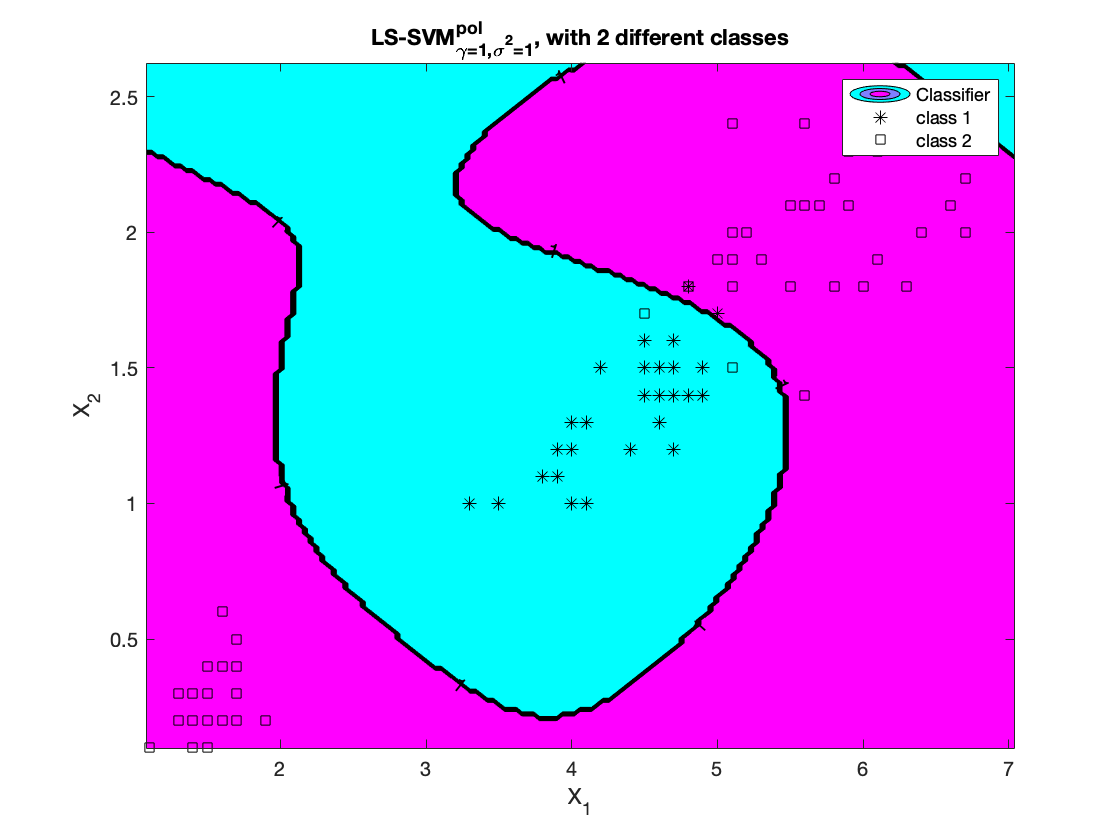
\includegraphics[width=\linewidth]{images/ls_svm_poly_deg4.png}
            \caption{d = 4}
        \end{subfigure}
        \begin{subfigure}{0.33\linewidth}
            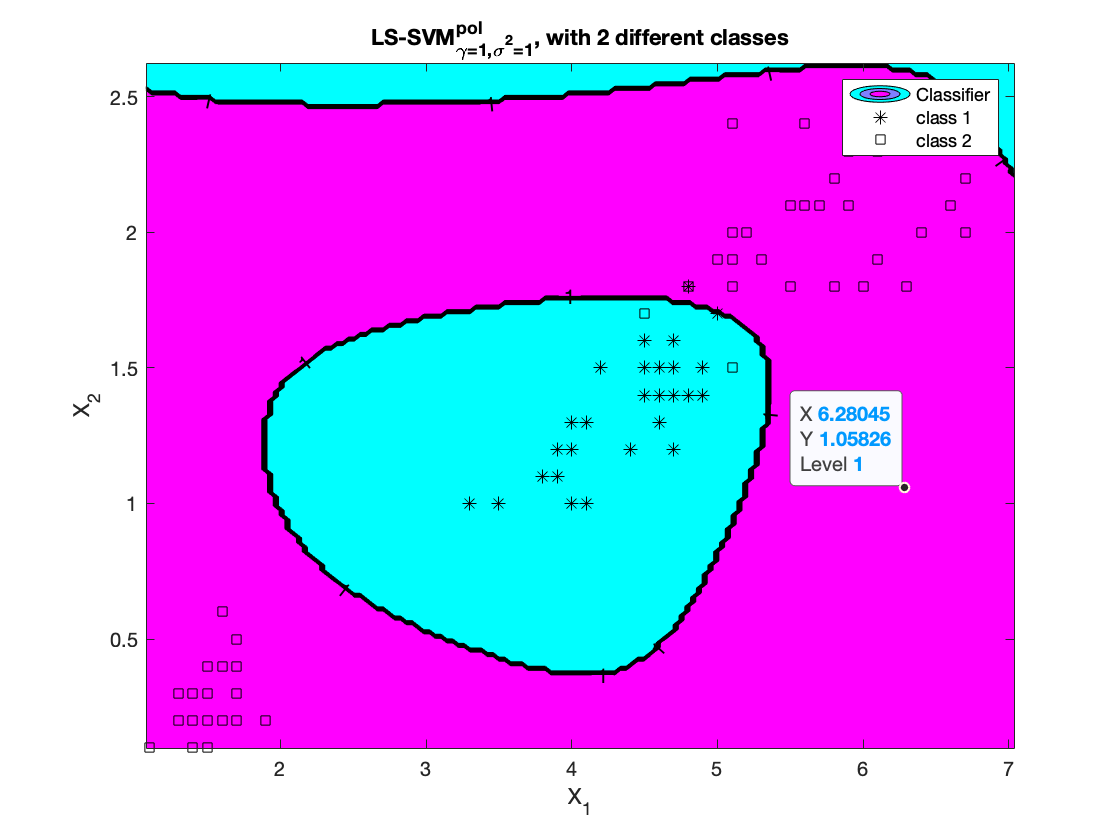
\includegraphics[width=\linewidth]{images/ls_svm_poly_deg5.png}
            \caption{d = 5}
        \end{subfigure}
        
        \begin{subfigure}{0.33\linewidth}
            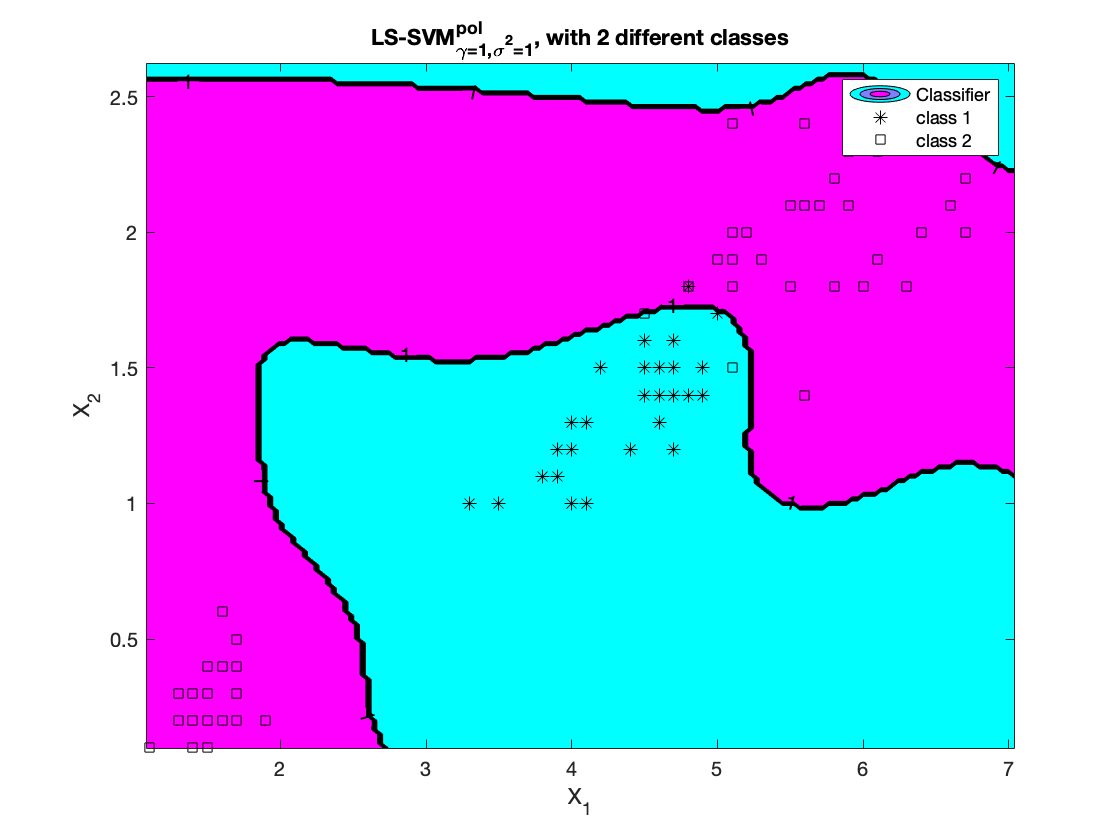
\includegraphics[width=\linewidth]{images/ls_svm_poly_deg10.png}
            \caption{d = 10}
        \end{subfigure}
        \begin{subfigure}{0.33\linewidth}
            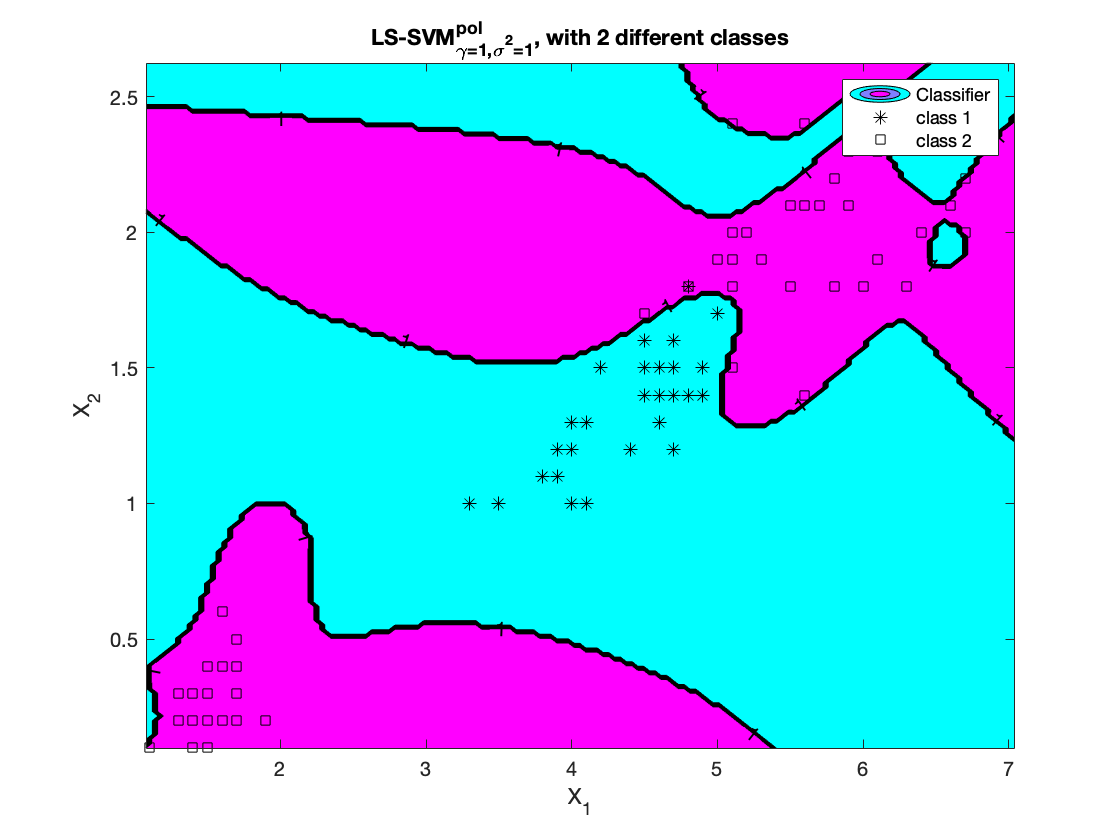
\includegraphics[width=\linewidth]{images/ls_svm_poly_deg15.png}
            \caption{d = 15}
        \end{subfigure}
        \begin{subfigure}{0.33\linewidth}
            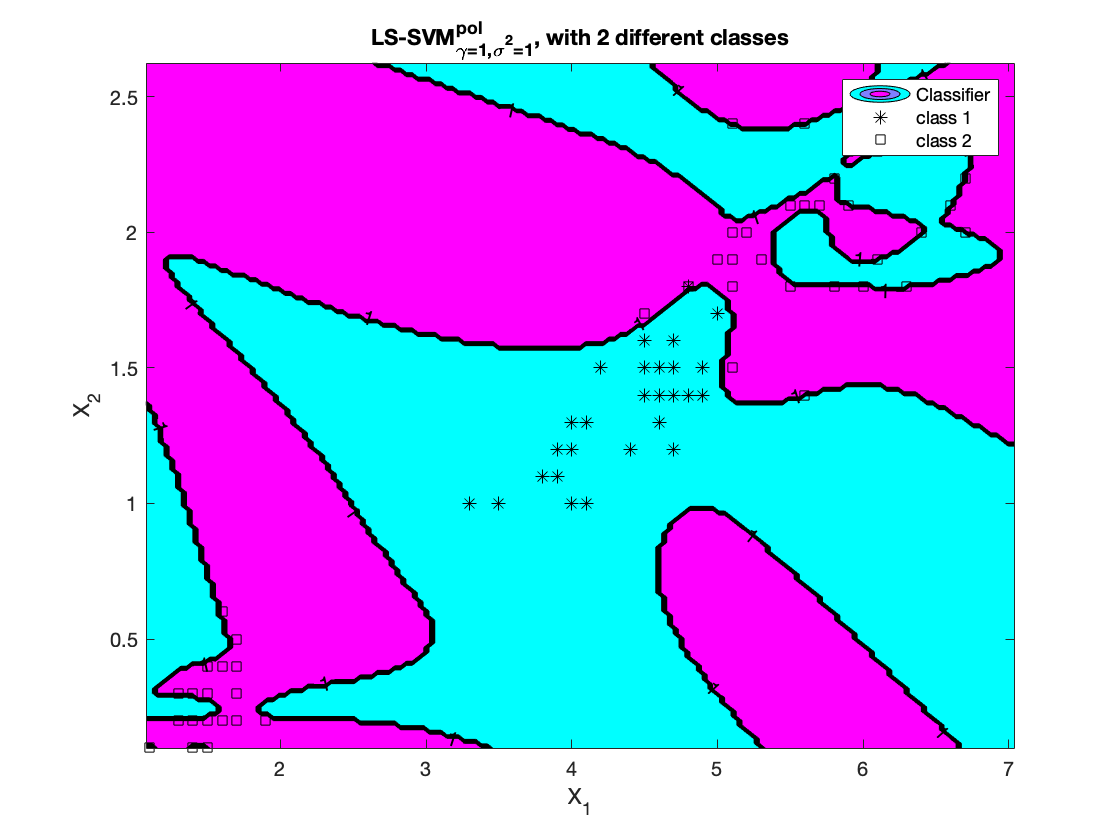
\includegraphics[width=\linewidth]{images/ls_svm._poly_deg20.png}
            \caption{d = 20}
        \end{subfigure}
  
        \caption{(a) linear kernel (b to i) different degrees on polynomial kernel}
        
        \label{fig:linpoly}
\end{figure*}

\begin{figure*}[]
        \begin{subfigure}{0.33\linewidth}
            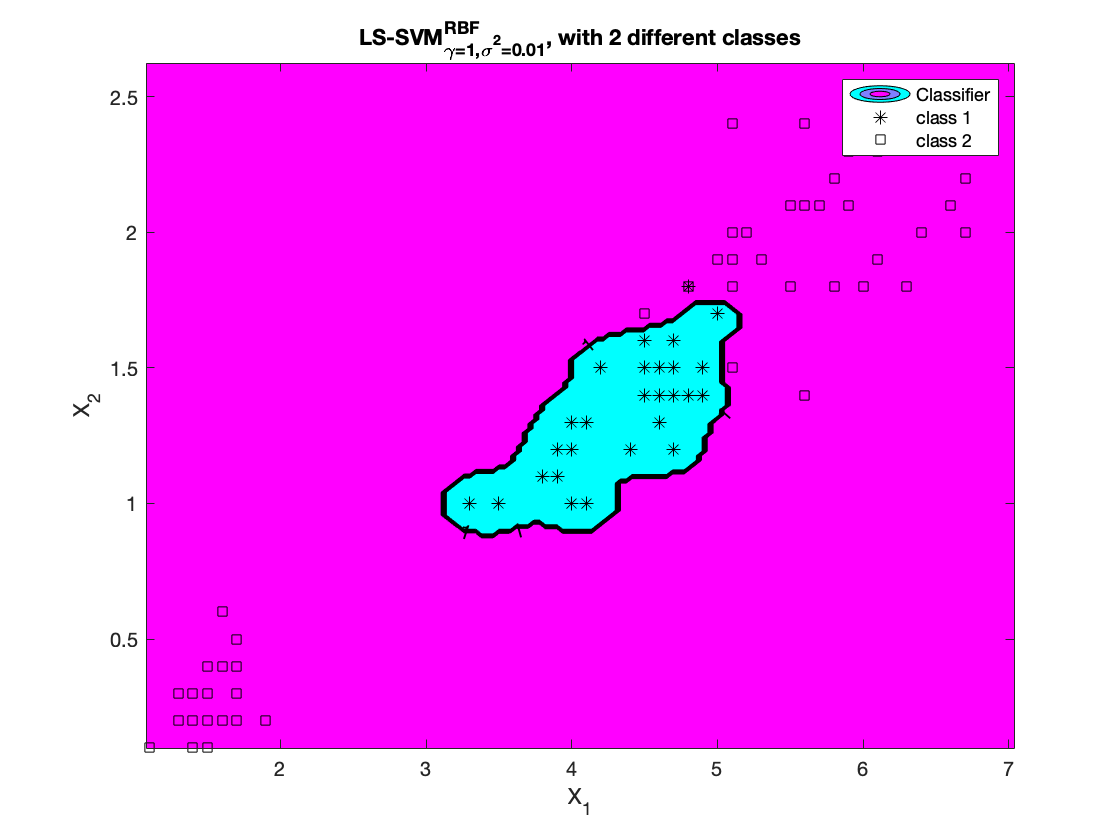
\includegraphics[width=\linewidth]{images/ls_svm_rbg_g1_s0.01.png}
            \caption{$\sigma^2=0.01$ and $\gamma=1$}
        \end{subfigure}
        \begin{subfigure}{0.33\linewidth}
            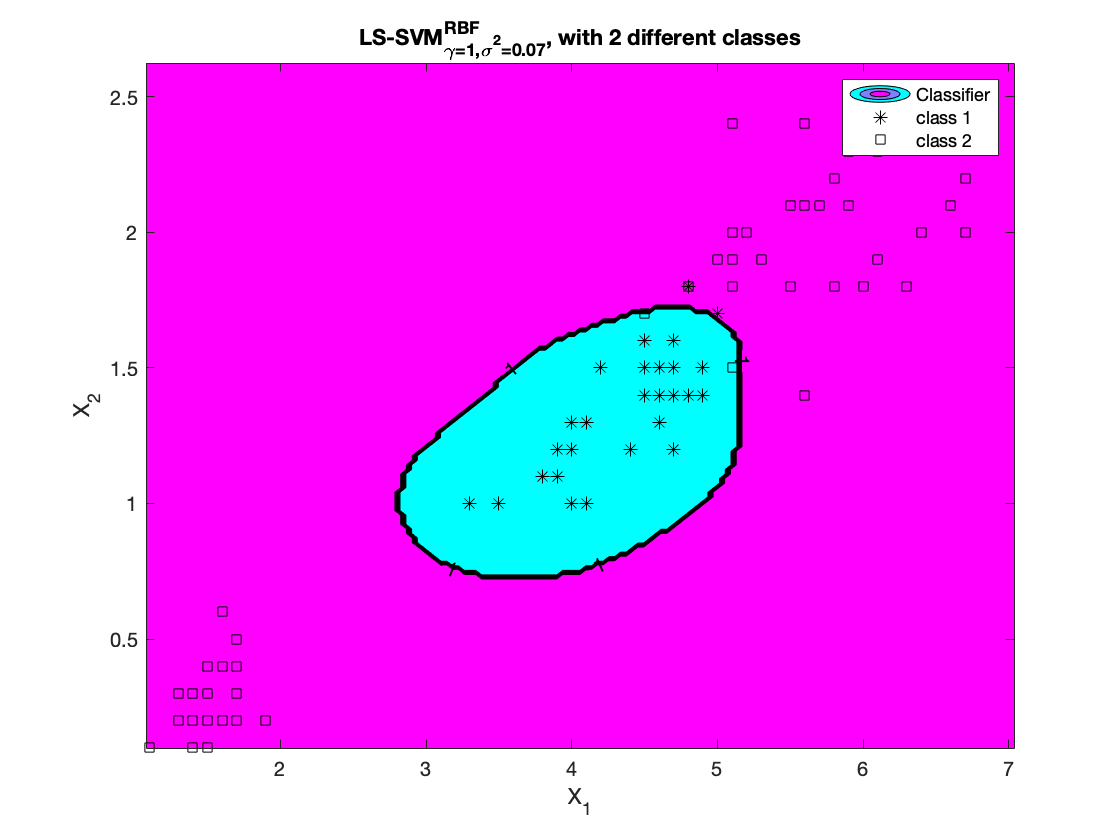
\includegraphics[width=\linewidth]{images/ls_svm_rbg_g1_s0.07.png}
            \caption{$\sigma^2=0.07$ and $\gamma=1$}
        \end{subfigure}
        \begin{subfigure}{0.33\linewidth}
            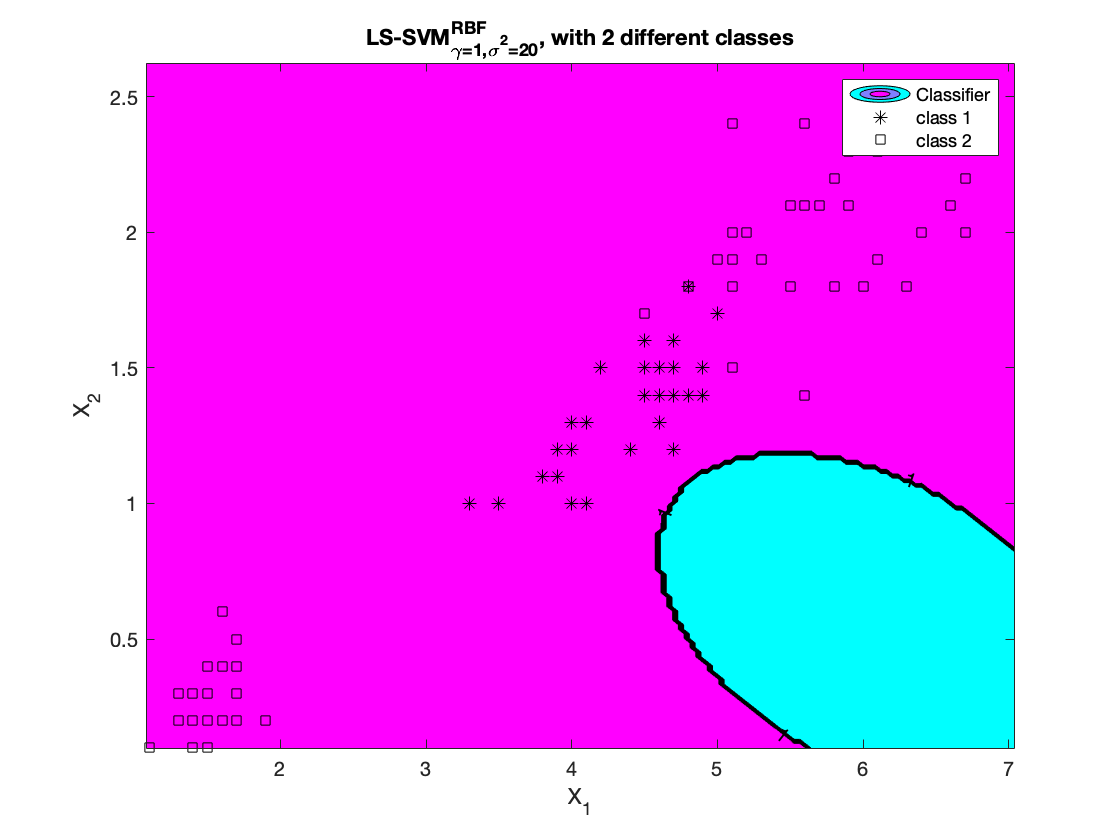
\includegraphics[width=\linewidth]{images/ls_svm_rbf_g1_s20.png}
            \caption{$\sigma^2=20$ and $\gamma=1$}
        \end{subfigure}

		\begin{subfigure}{0.33\linewidth}
            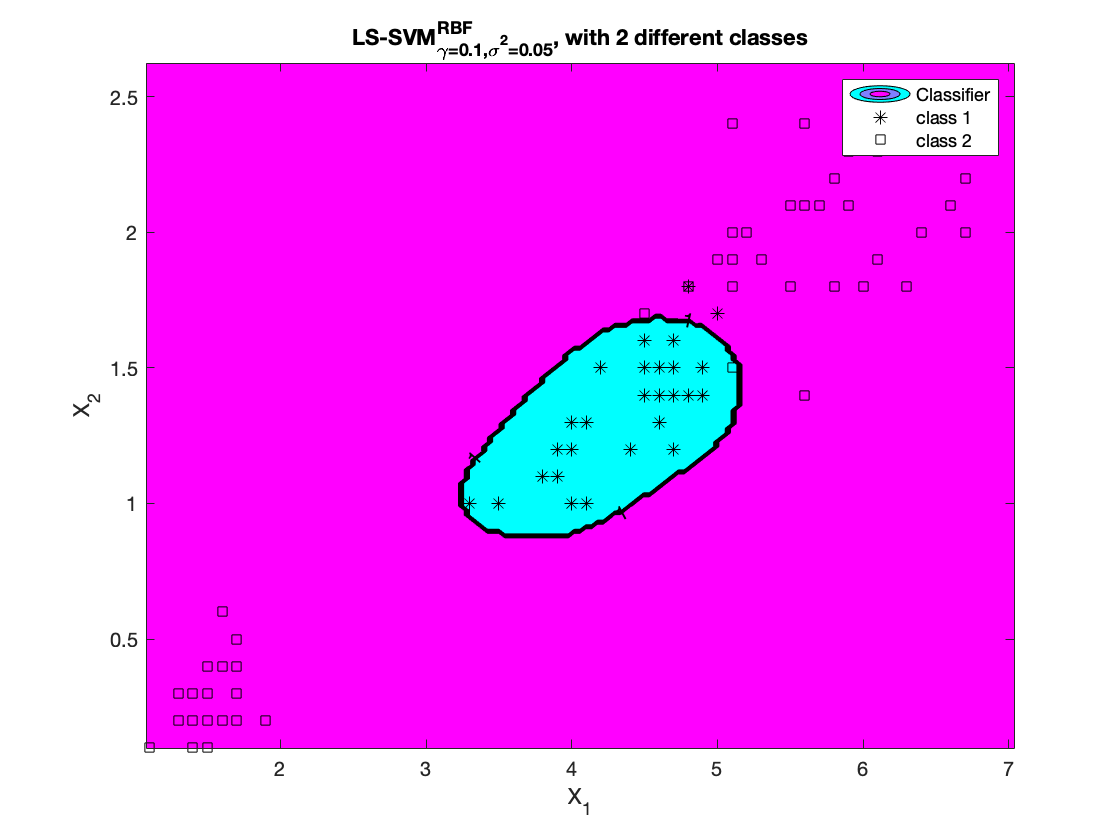
\includegraphics[width=\linewidth]{images/ls_svm_rbf_g0.1_s0.05.png}
            \caption{$\sigma^2=0.05$ and $\gamma=0.1$}
        \end{subfigure}
        \begin{subfigure}{0.33\linewidth}
            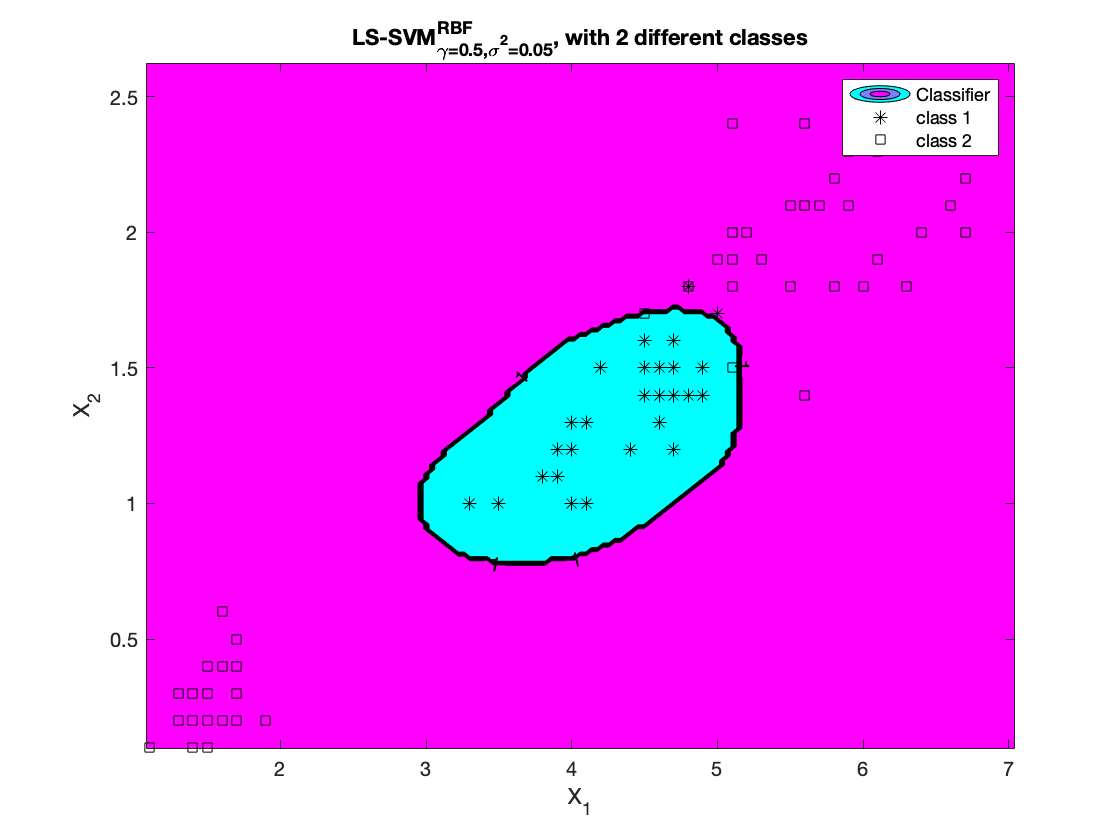
\includegraphics[width=\linewidth]{images/ls_svm_rbf_g0.5_s0.05.png}
            \caption{$\sigma^2=0.05$ and $\gamma=0.5$}
        \end{subfigure}
        \begin{subfigure}{0.33\linewidth}
            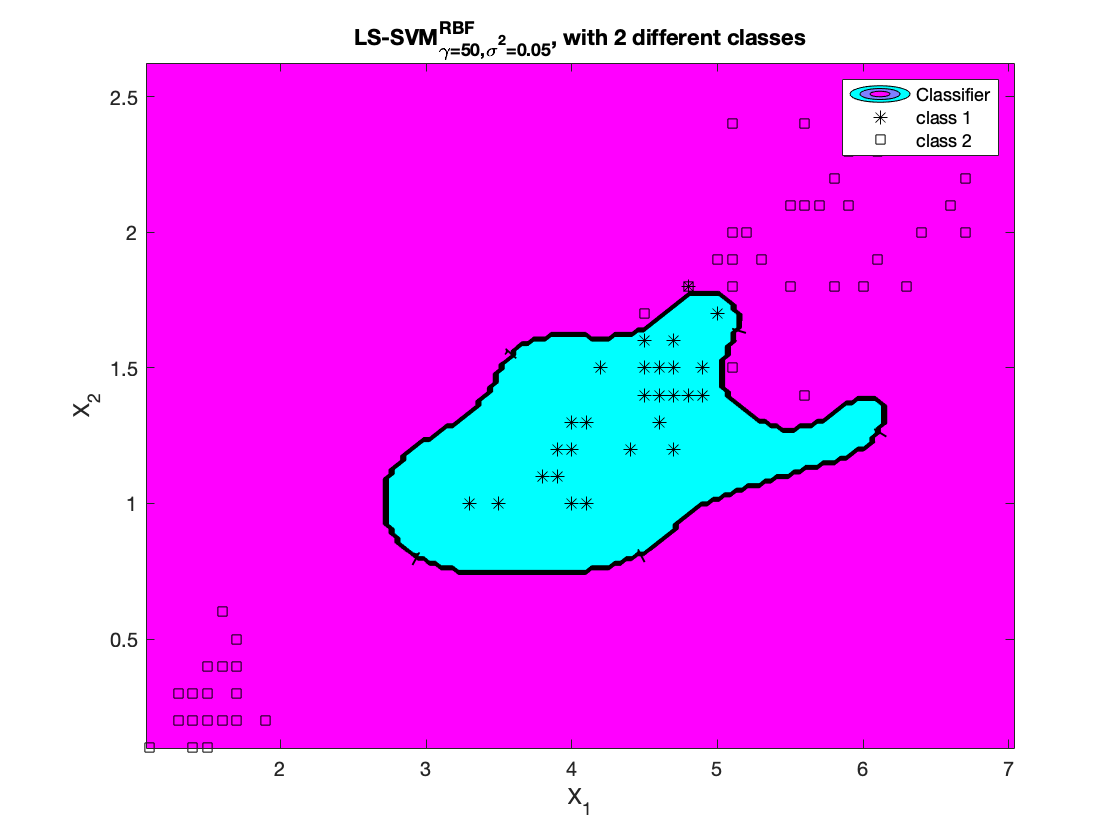
\includegraphics[width=\linewidth]{images/ls_svm_rbf_g50_s0.05.png}
            \caption{$\sigma^2=0.05$ and $\gamma=50$}
        \end{subfigure}
        \caption{Varying $\sigma^2$ and $\gamma$  in the RBF kernel.}       
        \label{fig:rbfvarcsigma}
    \end{figure*}


\subsubsection{Tuning parameters using validation}
In this section, the objective is to experiment with three different automated tuning methods and evaluate their performance. These automated tuning methods split the dataset into a training and validation set. 

\textbf{Random Split}
In random split, the dataset is randomly split into a training and a validation set. In order to evaluate the model the validation set is used. In contrast to a test set, the validation set is not meant to measure the performance of a fully specified model. The validation set is comprised of data independet of the ones used in the training and test sets, therefore it enables the model to be able to generalize more. One major issue of this method is that since the split is random, it may not be able to perform well when the dataset is too small. Additionally, the model is highly susceptible to the choice of data over which it is evaluated. 

\textbf{K-fold cross validation}
In k-fold cross validation the given dataset is randomly split into $k$ subsets, each having an equal size. The model is trained in $k-1$ subsets and the remaining subset after the split is used as the validation set. The same process is then repeated k times and every time the training and validation subsets switch. Finally, the created subsets are averaged and an estimation is obtained in order to evaluate the performance. In general, a specific number which is ideal for $k$ does not exist; however, it has been observed that a relatively low $k$ results in lower variance and higher bias, whereas a higher $k$ increases the variance but reduces the bias. 

\textbf{Leave-one-out validation}
Leave-one-out validation is a special case of k-fold cross validation, in which the number of all training examples $X$ is assigned the number of $k$. Training of the model is performed on all the available data $X$ times and the errors are averaged in order to measure the performance. A drawback of leave-one-out validation is that in large dataset it can affect the performance since it will require a high number of training data. 

\begin{figure*}[]
        \begin{subfigure}{0.33\linewidth}
            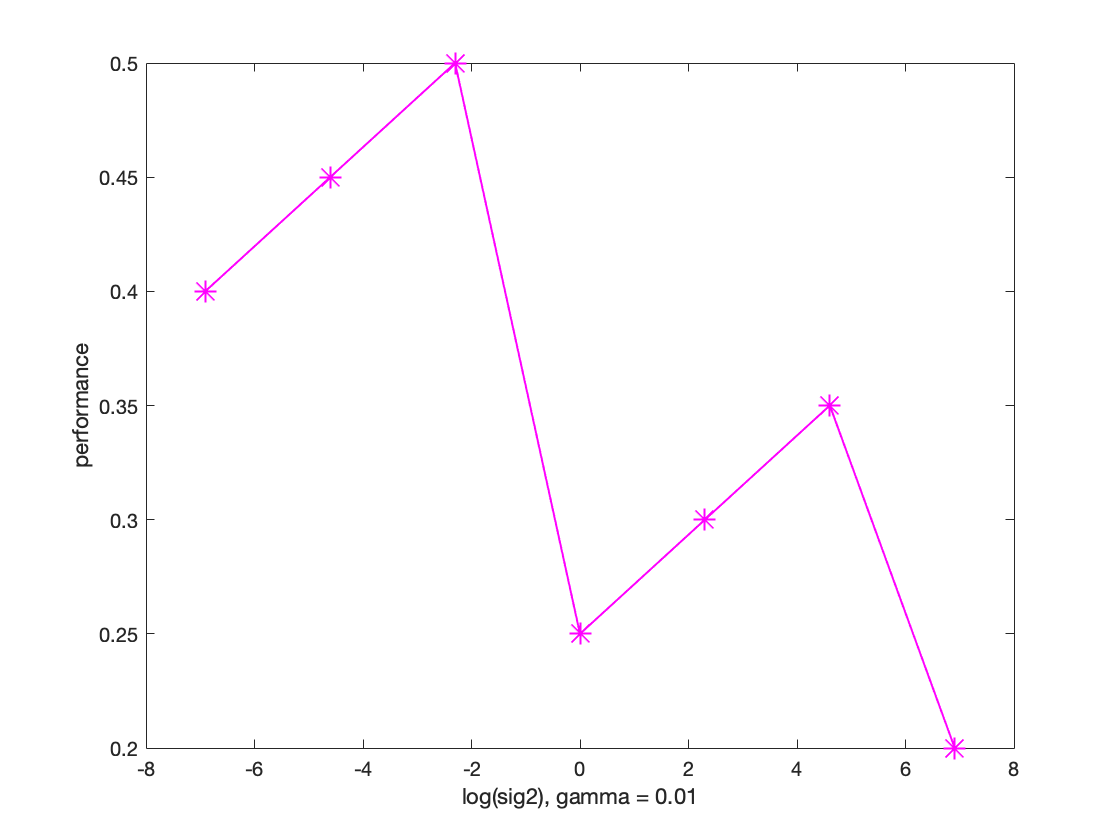
\includegraphics[width=\linewidth]{images/rsplit_0.01.png}
            \caption{$\sigma$ and $\gamma$ equal to $0.1$}
        \end{subfigure}
        \begin{subfigure}{0.33\linewidth}
            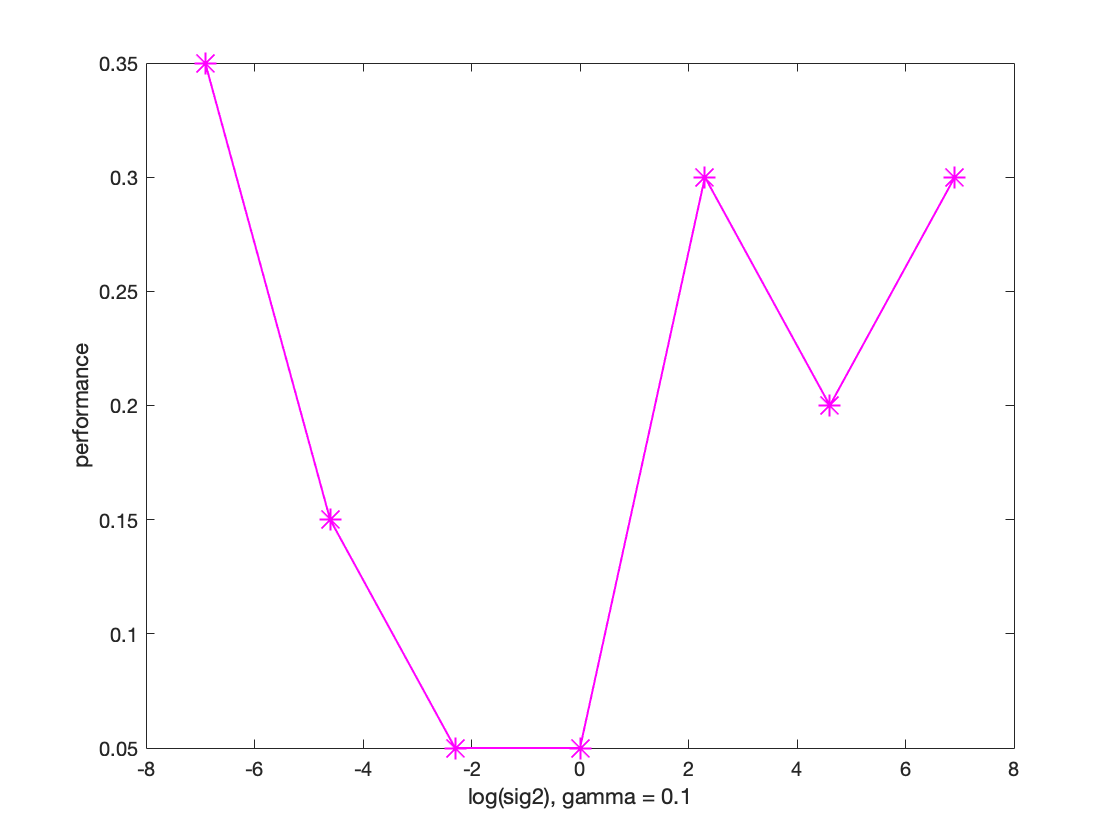
\includegraphics[width=\linewidth]{images/rsplit_0.1.png}
            \caption{$\sigma$ and $\gamma$ equal to $1$}
        \end{subfigure}
        \begin{subfigure}{0.33\linewidth}
            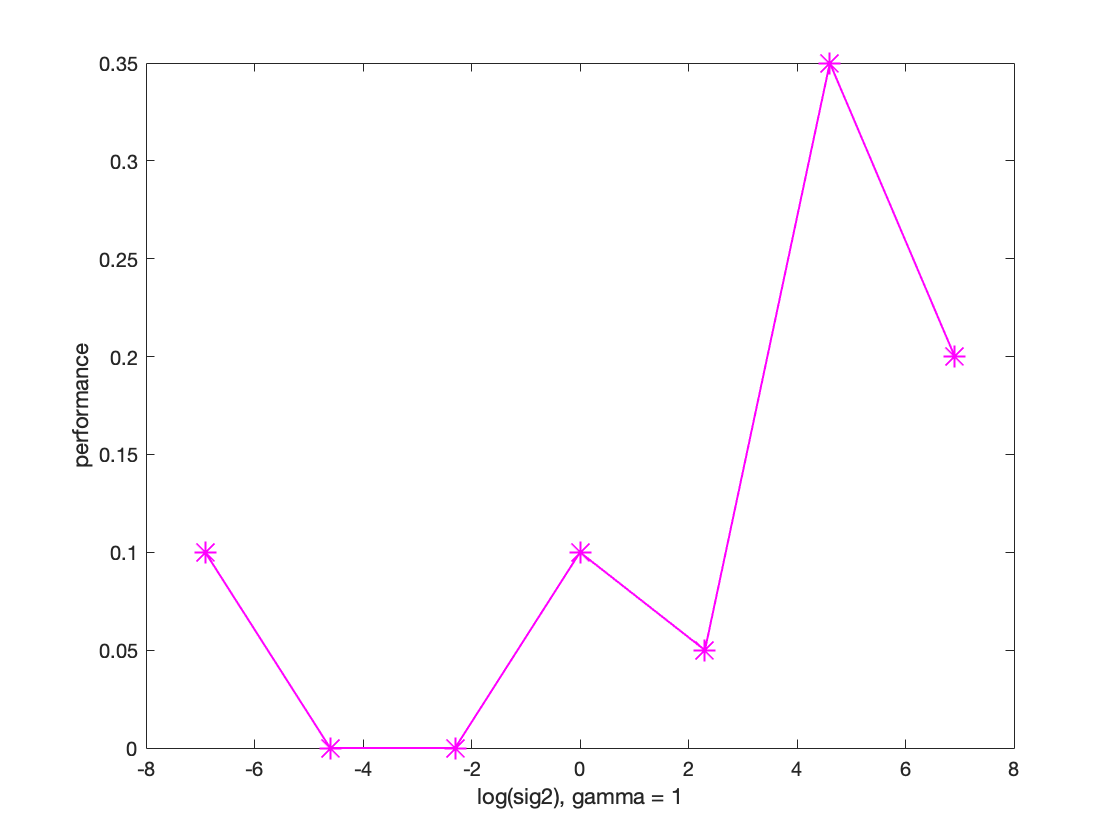
\includegraphics[width=\linewidth]{images/rsplit_1.png}
            \caption{$\sigma$ and $\gamma$ equal to $10$}
        \end{subfigure}
		\begin{subfigure}{0.33\linewidth}
            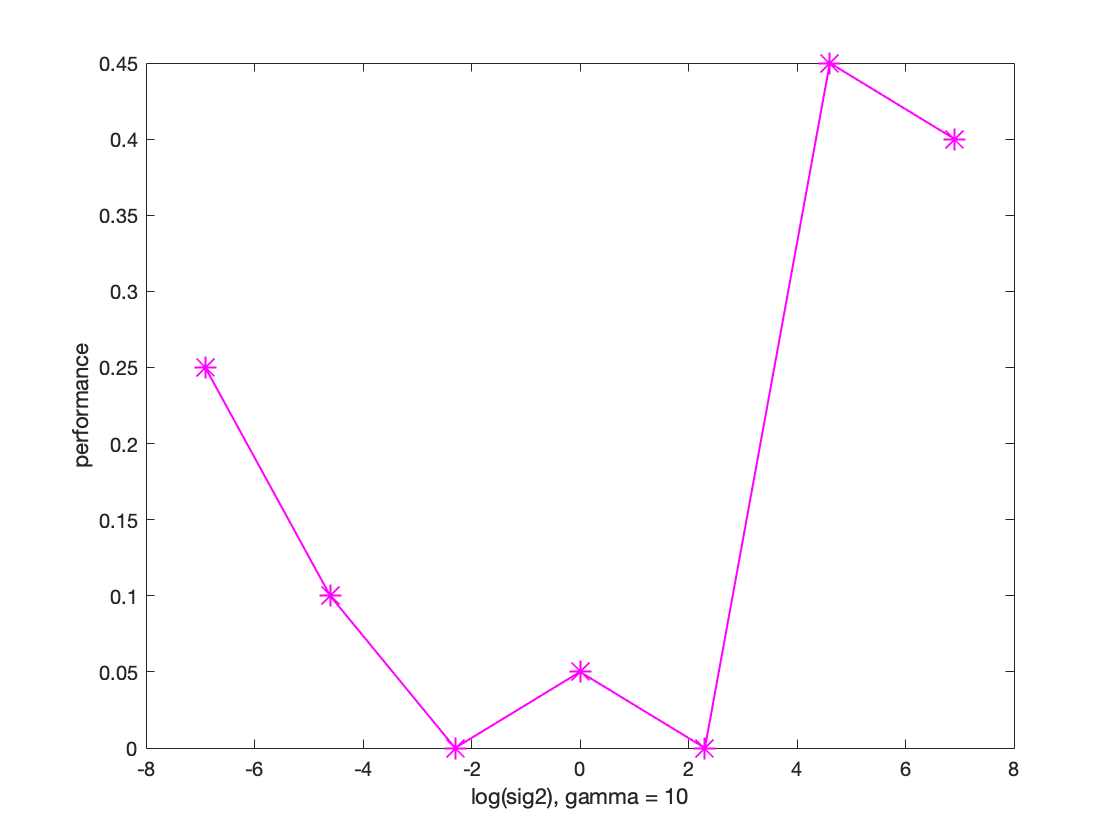
\includegraphics[width=\linewidth]{images/rsplit_10.png}
            \caption{$\sigma$ and $\gamma$ equal to $100$}
        \end{subfigure}
        \begin{subfigure}{0.33\linewidth}
            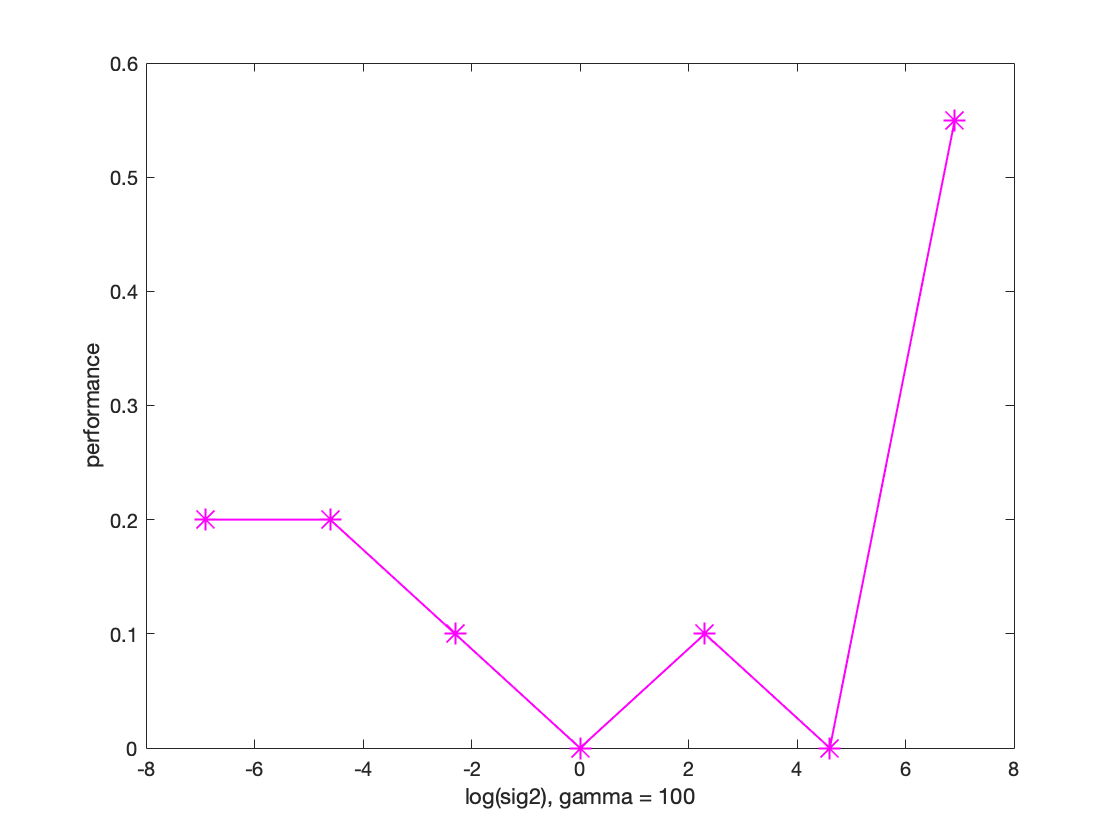
\includegraphics[width=\linewidth]{images/rsplit_100.png}
            \caption{$\sigma$ and $\gamma$ equal to $0.01$}
        \end{subfigure}
        \begin{subfigure}{0.33\linewidth}
            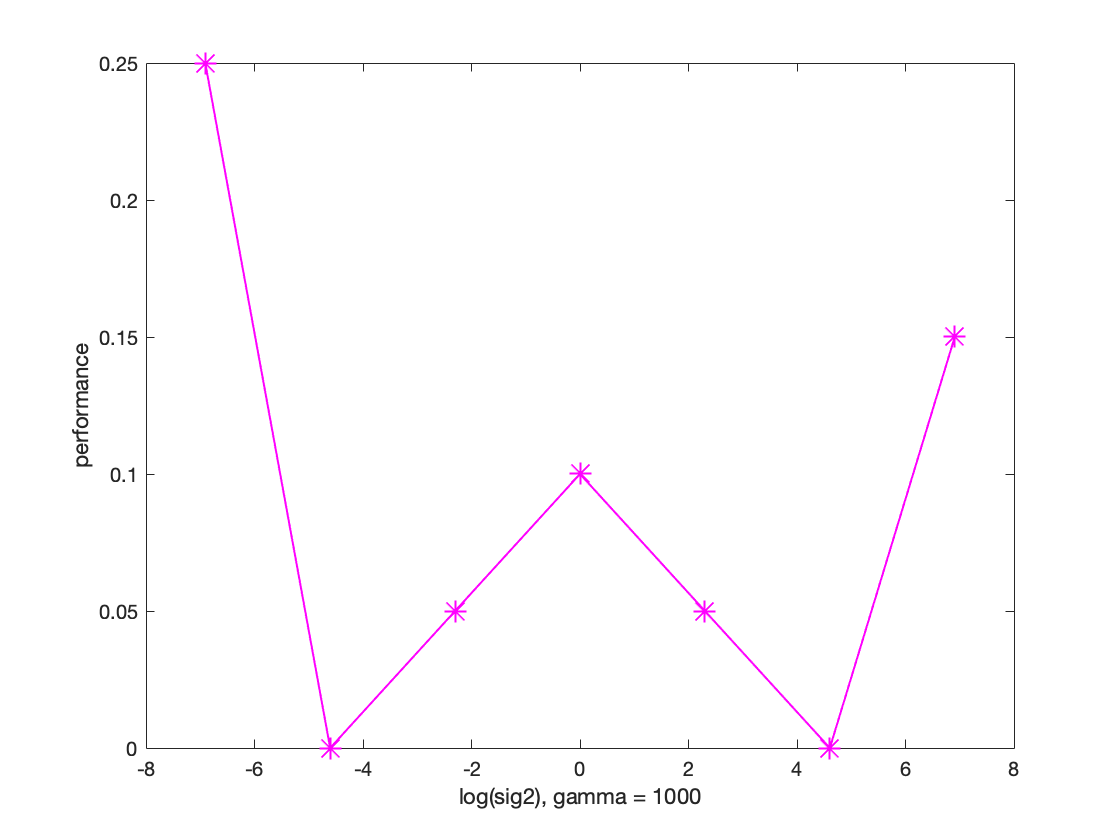
\includegraphics[width=\linewidth]{images/rsplit_1000.png}
            \caption{$\sigma$ and $\gamma$ equal to $1000$}
        \end{subfigure}
        \caption{Varying the values of $\sigma$ and $\gamma$ in random split}
        \label{fig:randomval}
\end{figure*}


\begin{figure*}[]
        \begin{subfigure}{0.33\linewidth}
            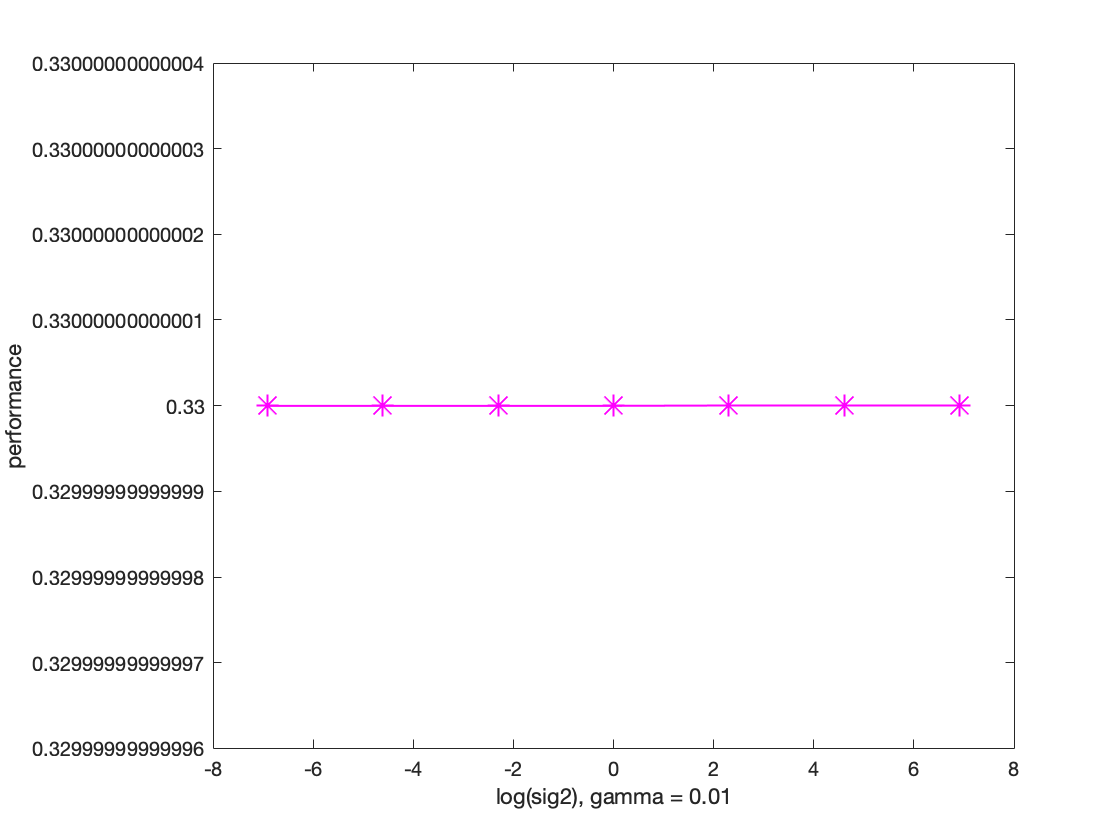
\includegraphics[width=\linewidth]{images/10f_sig2_g_0.01.png}
            \caption{$\sigma$ and $\gamma$ equal to $0.01$}
        \end{subfigure}
        \begin{subfigure}{0.33\linewidth}
            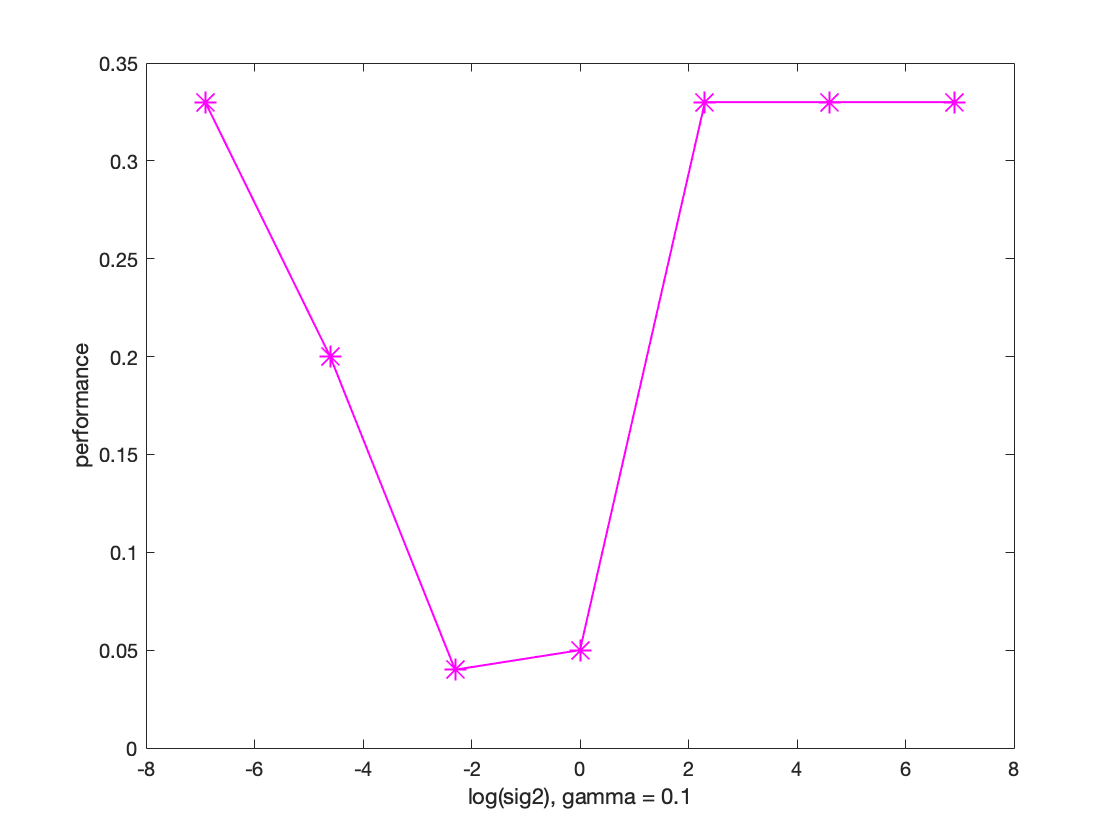
\includegraphics[width=\linewidth]{images/10f_sig2_g_0.1.png}
            \caption{$\sigma$ and $\gamma$ equal to $0.1$}
        \end{subfigure}
        \begin{subfigure}{0.33\linewidth}
            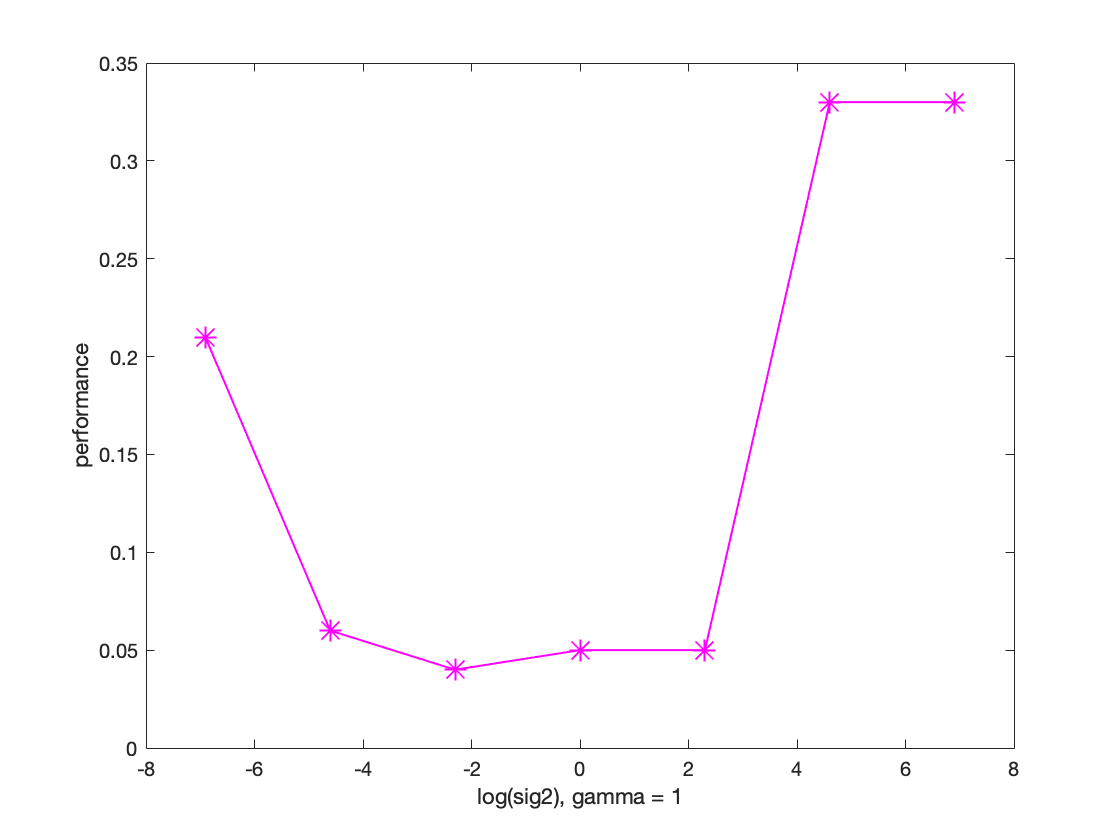
\includegraphics[width=\linewidth]{images/10f_sig2_g_1.png}
            \caption{$\sigma$ and $\gamma$ equal to $1$}
        \end{subfigure}
        \begin{subfigure}{0.33\linewidth}
            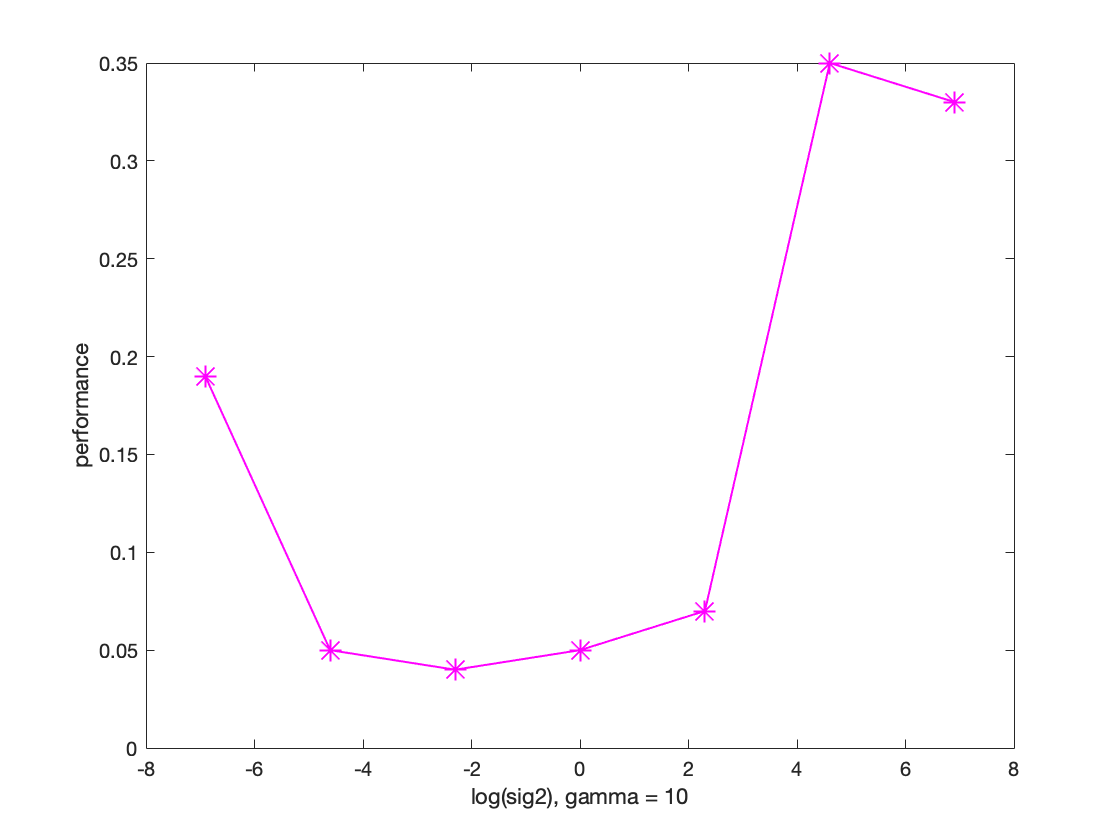
\includegraphics[width=\linewidth]{images/10f_sig2_g_10.png}
            \caption{$\sigma$ and $\gamma$ equal to $10$}
        \end{subfigure}
		\begin{subfigure}{0.33\linewidth}
            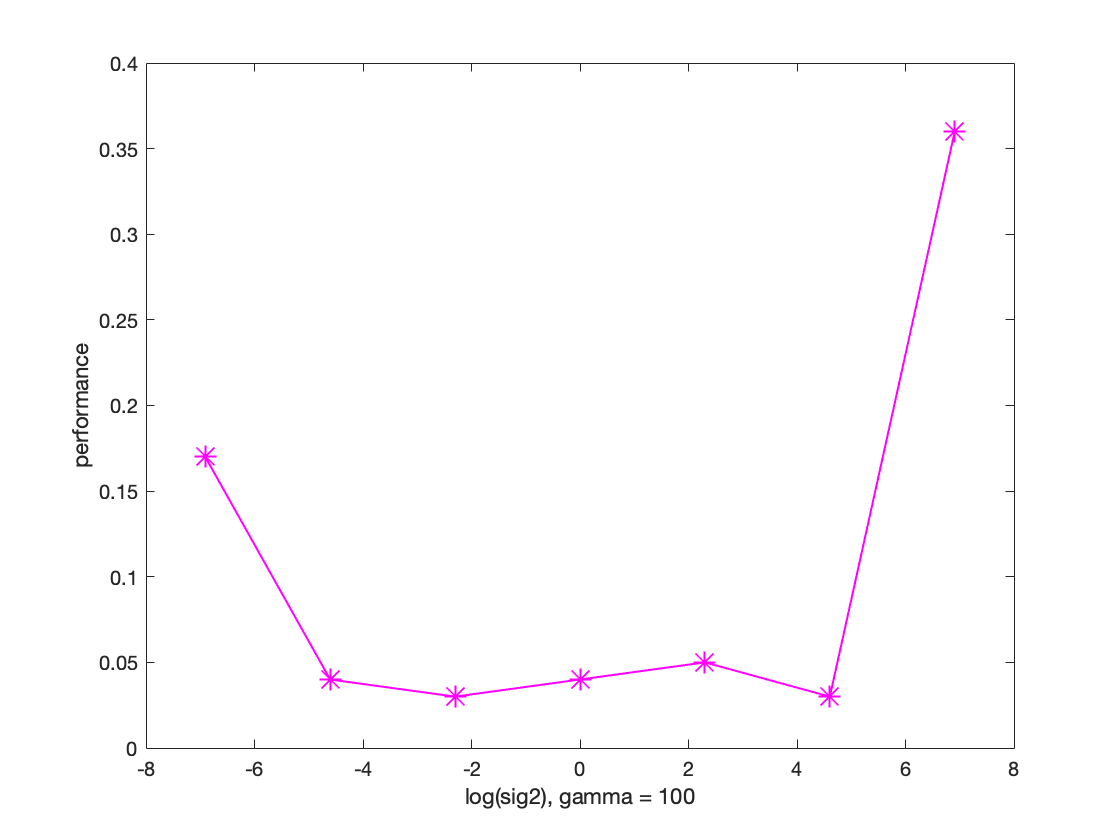
\includegraphics[width=\linewidth]{images/10f_sig2_g_100.png}
            \caption{$\sigma$ and $\gamma$ equal to $100$}
        \end{subfigure}
        \begin{subfigure}{0.33\linewidth}
            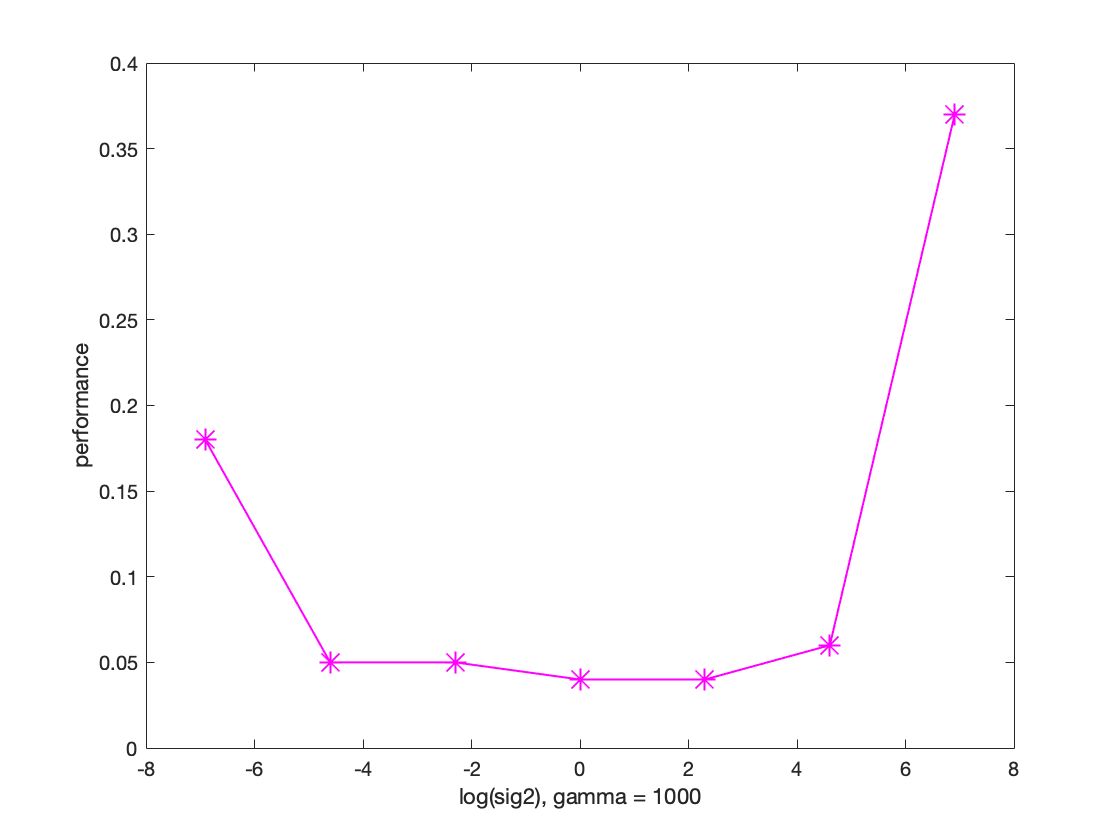
\includegraphics[width=\linewidth]{images/10f_sig2_g_1000.png}
            \caption{$\sigma$ and $\gamma$ equal to $1000$}
        \end{subfigure}
        \caption{Varying the values of $\sigma$ and $\gamma$ in 10-fold}
        \label{fig:kfoldval}
\end{figure*}

\begin{figure*}[]
        \begin{subfigure}{0.33\linewidth}
            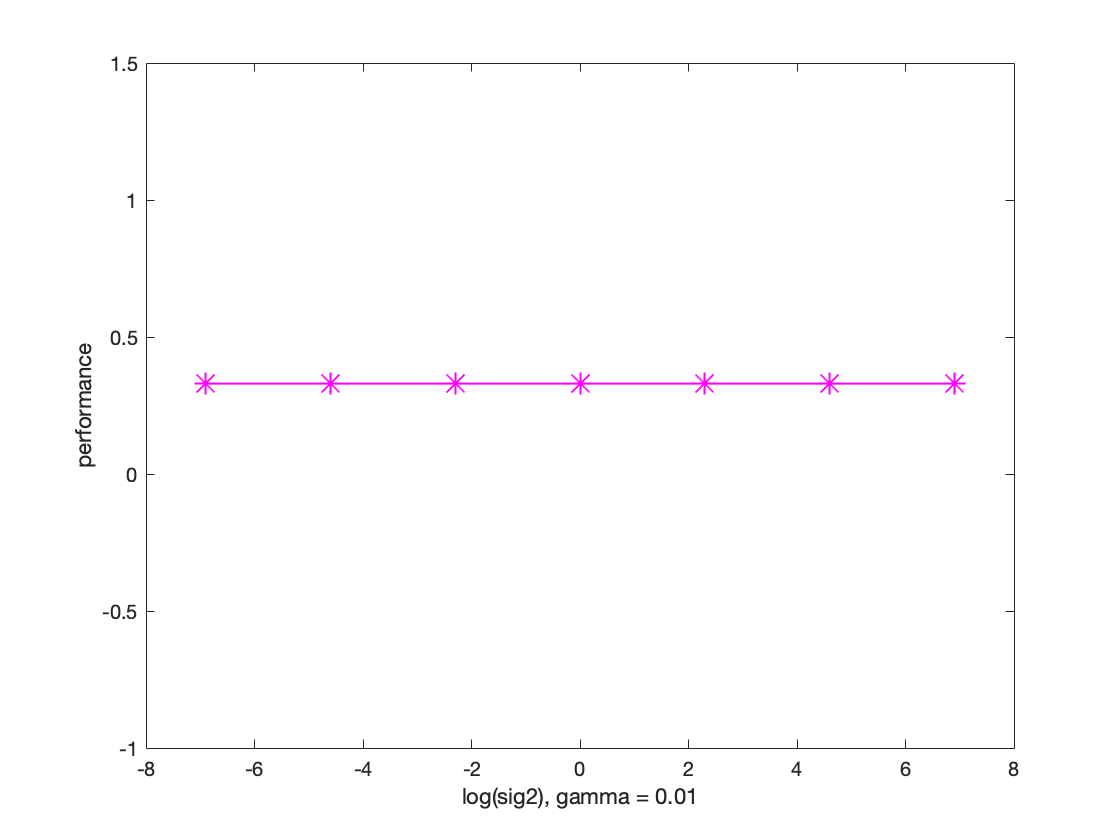
\includegraphics[width=\linewidth]{images/loo_sig2_g_0.01.png}
            \caption{$\sigma$ and $\gamma$ equal to $0.1$}
        \end{subfigure}
        \begin{subfigure}{0.33\linewidth}
            \includegraphics[width=\linewidth]{images/loo_sig2_g_0.1.png}
            \caption{$\sigma$ and $\gamma$ equal to $1$}
        \end{subfigure}
        \begin{subfigure}{0.33\linewidth}
            \includegraphics[width=\linewidth]{images/loo_sig2_g_1.png}
            \caption{$\sigma$ and $\gamma$ equal to $10$}
        \end{subfigure}
		\begin{subfigure}{0.33\linewidth}
            \includegraphics[width=\linewidth]{images/loo_sig2_g_10.png}
            \caption{$\sigma$ and $\gamma$ equal to $100$}
        \end{subfigure}
        \begin{subfigure}{0.33\linewidth}
            \includegraphics[width=\linewidth]{images/loo_sig2_g_100.png}
            \caption{$\sigma$ and $\gamma$ equal to $0.01$}
        \end{subfigure}
        \begin{subfigure}{0.33\linewidth}
            \includegraphics[width=\linewidth]{images/loo_sig2_g_1000.png}
            \caption{$\sigma$ and $\gamma$ equal to $1000$}
        \end{subfigure}
        \caption{Varying the values of $\sigma$ and $\gamma$ in leave-one-out}
        \label{fig:leaveoneval}
\end{figure*}

\subsubsection{Automatic parameter tuning}
In this section, two different algorithms (gridsearch and simplex) are tested in the task of automatic parameter tuning. These techniques are utilized in order to automatically tune the hyperparameters of a LS-SVM and are implemented in the provided LS-SVM toolbox\cite{Brabanter2003LSSVMlabTU}. Their results are summarized in Table\ref{fig:tbl1}. The Nelder-Mead method (simplex) is faster than gridsearch, taking almost half the time to complete the computations and obtain its parameters ($0.54$ and $0.9$ seconds respectively). Finally, we can observe a high variation in the hyperparameters everytime due to the fact that multiple minimum solutions may exist. 

\begin{table*}\centering
\begin{tabular}{@{}rrrrrrrccrrrcrrr@{}}\toprule
& \multicolumn{4}{c}{Simplex} & \phantom{abc}& \multicolumn{2}{c}{Gridsearch} &
\phantom{abc} \\
\cmidrule{1-5} \cmidrule{6-9} \cmidrule{10-12}
& $\gamma$ & $\sigma^2$ &     cost &&  $\gamma$ & $\sigma^2$ &    cost \\ \midrule
 &  2.4124 & 0.0658 &  0.043 && 0.340 & 0.9661 & 0.036 \\
\bottomrule
\end{tabular}
\caption{Hyperparameters tuned with Nelder-Mead method and Gridsearch for the classification task}
       \label{fig:tbl1}
\end{table*}



\subsubsection{Using ROC curves}
A Receiver Operating Characteristic (ROC) curve is used to measure the performance of a classifier. Specifically, a ROC curve expresses the relationship between specificity and sensitivity of a classifier. The sensitivity of a classifier is defined as 

\begin{equation}
TPR = \frac{TP}{TP+FN}
\end{equation}
where $TP$ and $FN$ (true positive and false negative) correspond to the number of correctly and incorrectly classified instances as positive. Sensitivity is also named as true positive rate.
The specificity of a classifier is defined as 
\begin{equation}
FPR = \frac{TN}{TN+FP}
\end{equation}
where $TN$ and $FP$ correspond to the number of correctly and incorrectly classified instances as negative. The Area Under the Curve (AUC) in a ROC curve describes the performance of the model. If it is close to $0$ then the model is able to separate the data perfectly, whereas if it is close to 0.5 the model behaves randomly. In Figure \ref{fig:ROCiris} we can see the ROC curve of the Iris dataset. 

\begin{figure*}[]
    \centering
    \includegraphics[width=12cm]{images/simplex_ROC_dataset.png}
    \caption{ROC curve of the Iris dataset}
    \label{fig:ROCiris}
\end{figure*}


\subsubsection{Bayesian framework}
In this section we experiment with using the Bayesian framework\cite{VanGestelTony2002Bffl} to get probability estimates. In Figure \ref{fig:bayesian_report1} we can see the illustration of the bayesian framework. The color represents the probability of an instance to belong to the positive class. Therefore, the blue color can be interpreted as the probability of the instance belonging to the positive class being close to zero, whereas magenta represents the opposite. 

\begin{figure*}[]
    \centering
    \includegraphics[width=12cm]{images/bay_plot_colorbar.png}
    \caption{Bayesian framework probabilistic view}
    \label{fig:bayesian_report1}
\end{figure*}
%%% TODO second bayes plot
\subsection{Homework problems}
\subsubsection{Ripley dataset}
The Ripley dataset contains of a training set and a test set. The training set contains $250$ datapoints for training and $1000$ datapoints for testing the model. As we can see in Figure \ref{fig:ripleymisc} (e) the two classes are quite, although not fully, separated from each other. Additionally, the results of applying a linear kernel and an RBF kernel are similar ($0.959$ and $0.968$ respectively) and are visualized in the ROC curves (c) and (d). The tuning of the hyperparameters for the RBF kernel were obtained after using the Nelder-Mead method which was discussed in section $1.3.3$.  

\begin{figure}[hbt]
        \begin{subfigure}{0.45\linewidth}
            \includegraphics[width=\linewidth]{images/ripley_linear.png}
            \caption{Linear kernel}
        \end{subfigure}
        \begin{subfigure}{0.45\linewidth}
            \includegraphics[width=\linewidth]{images/ripley_rbf_1.png}
            \caption{RBF kernel}
        \end{subfigure}
        \begin{subfigure}{0.45\linewidth}
            \includegraphics[width=\linewidth]{images/ripley_linearkernel_ROC.png}
            \caption{Linear kernel ROC}
        \end{subfigure}
        \begin{subfigure}{0.45\linewidth}
            \includegraphics[width=\linewidth]{images/ripley_ROC_RBF.png}
            \caption{RBF kernel ROC}
        \end{subfigure}
        \centering
	   \begin{subfigure}{0.45\linewidth}
            \includegraphics[width=\linewidth]{images/ripley_training.png}
            \caption{training set}
        \end{subfigure}
        \caption{Ripley dataset}        
        \label{fig:ripleymisc}
\end{figure}

\subsubsection{Wisconsin Breast Cancer dataset}
The Wisconsin Breast Cancer dataset is comprised of $569$ examples, $400$ for training and $169$ for testing purposes. Each datapoint is constructed from $30$ features that describe the metrics utilised for classification. The visualization of the dataset is illustrated in Figure \ref{fig:breastmisc}. As is illustrated in (c) and (d), the accuracy of the linear kernel is $0.9594$ and the accuracy of the RBF kernel is $0.98658$.


\begin{figure}[hbt]
        \begin{subfigure}{0.45\linewidth}
            \includegraphics[width=\linewidth]{images/breast_linearkernel.png}
            \caption{Linear kernel}
        \end{subfigure}
        \begin{subfigure}{0.45\linewidth}
            \includegraphics[width=\linewidth]{images/breast_training.png}
            \caption{Training set}
        \end{subfigure}
        \begin{subfigure}{0.45\linewidth}
            \includegraphics[width=\linewidth]{images/breast_linear_ROC.png}
            \caption{TLinear kernel ROC}
        \end{subfigure}
        \centering
        \begin{subfigure}{0.45\linewidth}
            \includegraphics[width=\linewidth]{images/breast_RBF_ROC.png}
            \caption{RBF kernel ROC}
        \end{subfigure}
        \caption{Wisconsin Breast Cancer dataset}
        \label{fig:breastmisc}
\end{figure}

\subsubsection{Diabetes dataset}
The Diabetes dataset consists of $468$ examples in total, out of which $300$ are utilized for training and $168$ for testing the model. Each datapoint is constructed from $8$ features. The two classes have high overlap in their distribution as visualized in Figure \ref{fig:diabetes}. The accuracy of the linear kernel is $0.84327$.

\begin{figure}[hbt]
        \begin{subfigure}{0.45\linewidth}
            \includegraphics[width=\linewidth]{images/diabetes_training.png}
            \caption{Training set}
        \end{subfigure}
        \begin{subfigure}{0.45\linewidth}
            \includegraphics[width=\linewidth]{images/diabetes_linearkernel.png}
            \caption{Training set}
        \end{subfigure}
        \centering
        \begin{subfigure}{0.45\linewidth}
            \includegraphics[width=\linewidth]{images/diabetes_lin_ROC.png}
            \caption{Linear kernel ROC}
        \end{subfigure}
        \caption{Diabetes dataset}
        \label{fig:diabetes}
\end{figure}


\section{Exercise 2}
\subsection{Support vector machine for function estimation}
In this exercise we utilize the SVM toolbox in order to perform function estimation. In order to use an SVM to perform such a task, it needs to be extended to be able to solve linear and nonlinear function estimation problems. Specifically, extending an SVM classifier for a regression task is done as following:

\begin{equation}
\min\limits_{w,b,\xi_i} J(w,b) = \frac{1}{2}w^Tw + C \sum_{k=1}^{N}(\xi_i)
\end{equation}

with 

\begin{equation}
    |y_i - w_ix_i| \leq \epsilon-\xi_i 
\end{equation}

The regularization parameter $C$ (also known as Bound), as discussed in the previous exercise session, is the parameter that determines the influence of misclassification on the objective function. As $C$ increases we can obtain more datapoints outside the area of $\epsilon$, which is the value responsible for controlling the sparsity (number of support vectors) of the resulting solution. Increasing the value of $\epsilon$ to relatively high numbers results in less support vectors, therefore the accuracy of the function approximation is less accurate. 
The initial dataset and the applied kernels are illustrated in Figure \ref{fig:simplelineardataset}.
Initially, we construct a dataset that will be utilized for a linear kernel SVM and next we construct a more complex dataset. Both datasets are comprised of around $20$ points and different kernels are tested for each dataset. 

In Figure \ref{fig:decreasingc} we can see that while decreasing the bound, the model tends to become more smooth and more sparse. Conversely, when $\epsilon$ decreases, the model becomes less sparse and the approximation more smooth. This is illustrated in Figure \ref{fig:decreasinge}.  

\begin{figure*}[]
        \begin{subfigure}{0.33\linewidth}
            \includegraphics[width=\linewidth]{images/linear_e=0.png}
            \caption{Linear kernel}
        \end{subfigure}\hfil
        \begin{subfigure}{0.33\linewidth}
            \includegraphics[width=\linewidth]{images/RBF_e=0.png}
            \caption{RBF kernel}
        \end{subfigure}\hfil
        \centering
        \begin{subfigure}{0.33\linewidth}
            \includegraphics[width=\linewidth]{images/poly_3=0.png}
            \caption{Polynomial kernel}
        \end{subfigure}\hfil
        \begin{subfigure}{0.33\linewidth}
            \includegraphics[width=\linewidth]{images/MLP_e=0.png}
            \caption{MLP kernel}
        \end{subfigure}\hfil
        \caption{Applying different kernels to the dataset}
        \label{fig:simplelineardataset}
\end{figure*}


\begin{figure*}[]
        \begin{subfigure}{0.33\linewidth}
            \includegraphics[width=\linewidth]{images/rbf_2_c_0.01.png}
            \caption{$c=0.01$}
        \end{subfigure}\hfil
        \begin{subfigure}{0.33\linewidth}
            \includegraphics[width=\linewidth]{images/rbf_2_c_0.1.png}
            \caption{$c=0.1$}
        \end{subfigure}\hfil
        \begin{subfigure}{0.33\linewidth}
            \includegraphics[width=\linewidth]{images/rbf_2_c_1.png}
            \caption{$c=1$}
        \end{subfigure}\hfil
        \begin{subfigure}{0.33\linewidth}
            \includegraphics[width=\linewidth]{images/rbf_2_c_10.png}
            \caption{$c=10$}
        \end{subfigure}\hfil
        \begin{subfigure}{0.33\linewidth}
            \includegraphics[width=\linewidth]{images/rbf_2_c_100.png}
            \caption{$c=100$}
        \end{subfigure}\hfil
        \begin{subfigure}{0.33\linewidth}
            \includegraphics[width=\linewidth]{images/rbf_2_c_inf.png}
            \caption{$c=inf$}
        \end{subfigure}\hfil
        \caption{Varying $c$ with $\sigma$ fixed to 0.01}
        \label{fig:decreasingc}
\end{figure*}


\begin{figure*}[]
        \begin{subfigure}{0.33\linewidth}
            \includegraphics[width=\linewidth]{images/rbf_bound_100_e_0.01.png}
            \caption{$\sigma = 0.01$}
        \end{subfigure}\hfil
        \begin{subfigure}{0.33\linewidth}
            \includegraphics[width=\linewidth]{images/rbf_bound_100_e_0.05.png}
            \caption{$\sigma = 0.05$}
        \end{subfigure}\hfil
        \centering
        \begin{subfigure}{0.33\linewidth}
            \includegraphics[width=\linewidth]{images/rbf_bound_100_e_0.09.png}
            \caption{$\sigma = 0.09$}
        \end{subfigure}\hfil
        \begin{subfigure}{0.33\linewidth}
            \includegraphics[width=\linewidth]{images/rbf_bound_100_e_0.5.png}
            \caption{$\sigma = 0.5$}
        \end{subfigure}\hfil
        \caption{Varying $\sigma$ with $c$ fixed to 100}
        \label{fig:decreasinge}
\end{figure*}

\subsection{The sinc function}
\subsubsection{Regression of the sinc function}
The objective of this exercise is to approximate the function
\begin{equation}
    y = sinc (x) + \epsilon
\end{equation}
 Initially, we construct an artificial dataset from the $sinc$ function. Next, we manually test the model for varying values of $c$ and $\sigma^2$. The model that achieved the lowest MSE score ($0.013$) was initialised with $c=10^6$ and $\sigma^2=1$. In Figure \ref{fig:sincfixsigma} we can see various values for $c$ with a fixed $\sigma=1$ whereas Figure \ref{fig:sincfixc} illustrates various values for $\sigma$ with a fixed $c=10^6$.
In the second part of the exercise, we use autotuning of the hyperparameters with 10-fold crossvalidation. Similarly to the previous exercise session, the methods utilized for automated hyperparameter tuning are the Nelder-Mead method (simplex) and gridsearch. We test the parameters obtained after $50$ runs and the results are aggregated in Table \ref{fig:tbl2}. %TODO tbl3 and tbl2 

\begin{table}[H]\centering
\begin{tabular}{@{}rrrrrrrccrrrcrrr@{}}\toprule
& \multicolumn{4}{c}{Simplex} & \phantom{abc}& \multicolumn{2}{c}{Gridsearch} &
\phantom{abc} \\
\cmidrule{1-5} \cmidrule{6-9} \cmidrule{10-12}
& $\gamma$ & $\sigma^2$ &     cost &&  $\gamma$ & $\sigma^2$ &    cost \\ \midrule
 &  197.57 & 0.1798 &  0.0196 && 103.81 & 0.2661 & 0.019 \\
\bottomrule
\end{tabular}
\caption{Hyperparameters tuned with Nelder-Mead method and Gridsearch for the regression task}
       \label{fig:tbl2}
\end{table}



\begin{figure}[H]
    \centering
        \begin{subfigure}{0.33\linewidth}
            \includegraphics[width=6.5cm]{images/sig1_gamma_0.01.png}
            \caption{$c=0.01$}
        \end{subfigure}\hfil
        \begin{subfigure}{0.33\linewidth}
            \includegraphics[width=6.5cm]{images/sig1_gamma_0.1.png}
            \caption{$c=0.1$}
        \end{subfigure}\hfil
        \begin{subfigure}{0.33\linewidth}
            \includegraphics[width=6.5cm]{images/sig1_gamma_1.png}
            \caption{$c=1$}
        \end{subfigure}\hfil
        \begin{subfigure}{0.33\linewidth}
            \includegraphics[width=6.5cm]{images/sig1_gamma_10.png}
            \caption{$c=10$}
        \end{subfigure}\hfil
        \begin{subfigure}{0.33\linewidth}
            \includegraphics[width=6.5cm]{images/sig1_gamma_100.png}
            \caption{$c=100$}
        \end{subfigure}\hfil
        \begin{subfigure}{0.33\linewidth}
            \includegraphics[width=6.5cm]{images/sig1_gamma_1000.png}
            \caption{$c=10^3$}
        \end{subfigure}\hfil
        \begin{subfigure}{0.33\linewidth}
            \includegraphics[width=6.5cm]{images/sig1_gamma_10^6.png}
            \caption{$c=10^6$}
        \end{subfigure}\hfil
        \caption{Varying $c$ with $\sigma$ fixed to $1$}
        \label{fig:sincfixsigma}
\end{figure}


\begin{figure}[H]
    \centering
        \begin{subfigure}{0.33\linewidth}
            \includegraphics[width=6.5cm]{images/sig_0.01_gamma_10^6png.png}
            \caption{$\sigma=0.01$}
        \end{subfigure}\hfil
        \begin{subfigure}{0.33\linewidth}
            \includegraphics[width=6.5cm]{images/sig_0.1_gamma_10^6.png}
            \caption{$\sigma=0.1$}
        \end{subfigure}\hfil
        \begin{subfigure}{0.33\linewidth}
            \includegraphics[width=6.5cm]{images/sig_1_gamma_10^6.png}
            \caption{$\sigma=1$}
        \end{subfigure}\hfil
        \begin{subfigure}{0.33\linewidth}
            \includegraphics[width=6.5cm]{images/sig_10_gamma_10^6.png}
            \caption{$\sigma=10$}
        \end{subfigure}\hfil
        \begin{subfigure}{0.33\linewidth}
            \includegraphics[width=6.5cm]{images/sig_100_gamma_10^6.png}
            \caption{$\sigma=100$}
        \end{subfigure}\hfil
        \begin{subfigure}{0.33\linewidth}
            \includegraphics[width=6.5cm]{images/sig_1000_gamma_10^6.png}
            \caption{$\sigma=10^3$}
        \end{subfigure}\hfil
        \caption{Varying $\sigma$ with $c$ fixed to $10^6$}
        \label{fig:sincfixc}
\end{figure}


\subsubsection{Application of the Bayesian framework}
When working in a Bayesian learning setting datapoints are characterized by their probability distribution. In such a setting, we assigned a probability over all the possible values for a datapoint instead of treating it as an individual point. Therefore, we have a prior $p(w)$ distribution over data $D$ and a likelihood distribution $p(D|w)$ which describe the posterior probability distribution $p(w|D)$ as

\begin{equation}
     P(w|D)=\frac{P(D|w)P(w)}{P(D}
\end{equation}

Parameter tuning in a Bayesian network works on three different levels, determined by the Bayesian framework that applies the aforementioned rule. 

\textbf{Level 1}
In the first level,the parameters that are inferred are $w$ and $b$. In this level, we calculate the posterior distribution parameters, given by

\begin{equation}
p(w,b|D,\mu,\zeta,H_\sigma) = \frac{p(D|w,b,\mu,\zeta,H_\sigma)}{p(D|\mu,\zeta,H_\sigma}p(w,b|\mu,\zeta,H_\sigma)
\end{equation}

In the LSVM toolbox in particular, \textbf{crit\_L1} corresponds to the cost that is proportional to the posterior $p(w,b|D,\mu,\zeta,H_\sigma$. 

\textbf{Level 2}
In the second level, the parameters that are inferred are $\mu$ and $\zeta$, with $\gamma = \frac{\mu}{\zeta}$. They are inferred from

\begin{equation}
p(\mu,\zeta|D,\mu,H_\sigma) = \frac{p(D|\mu,\zeta,H_\sigma)}{p(D|H_\sigma)}p(\mu,\zeta|H_\sigma)
\end{equation}

In the LSVM toolbox these are calculated by \textbf{crit\_L2}. In order to optimize the posterior, we first need to find the optimal $\gamma$, which is calculated with $\gamma = \frac{\mu}{\zeta}$. This is obtained by using the \textbf{bay\_optimize} function.

\textbf{Level 3}
In the third level the parameters that are inferred are the kernel parameters. In the case of RBF, the distribution of the kernel parameters is defined as

\begin{equation}
    p(H_\sigma|D) = \frac{p(D|H_\sigma)}{p(D)}p(H_\sigma)
\end{equation}

where $H_\sigma$ corresponds to an RBF kernel with width $\sigma$.
\subsection{Automatic relevance determination}
Automatic relevance determination (ARD) is a method that is utilized in order to evaluate the relevance of the input features. In this exercise we apply ARD to a three-dimensional input ($X1$, $X2$, $X3$) in order to determine the most significant feature. After executing the program, the result is that $X1$ is the most relevant feature. Figure \ref{fig:ARD} illustrates (a) the initial situation and (b) the selected feature.

\begin{figure}[H]
    \centering
    \begin{subfigure}{0.33\linewidth}
            \includegraphics[width=\linewidth]{images/ARD_all.png}
            \caption{initial}
        \end{subfigure}\hfil
        \begin{subfigure}{0.33\linewidth}
            \includegraphics[width=\linewidth]{images/ARD_selected.png}
            \caption{selected}
        \end{subfigure}\hfil
    \caption{(a) Initial 3-dimensional distribution of X1, X2, X3 and (b)Distribution of most important feature X1}
    \label{fig:ARD}
\end{figure}

\subsection{Robust Regression}
In this section we investigate the effect of outliers on an LS-SVM classifier. In particular, new datapoints are added to Y and then we train two different LS-SVM models: (1) that does not take into account efficient handling of them (non-robust) and (2) a model that takes into account the outliers (robust). The two models behave differently which is to be expected due to the effect the outliers have in such tasks. The non-robust model reacts to the outliers and tries to approximate them instead of the function whereas the robust model is not greatly affected and approximates the function better. This is illustrated in Figure \ref{fig:robustregr}. 

\begin{figure}[H]
    \centering
    \begin{subfigure}{0.45\linewidth}
            \includegraphics[width=\linewidth]{images/non_robust.png}
            \caption{non-robust model}
        \end{subfigure}\hfil
        \begin{subfigure}{0.45\linewidth}
            \includegraphics[width=\linewidth]{images/robust.png}
            \caption{robust model}
        \end{subfigure}\hfil
    \caption{Illustration of the (a) non-robust and (b) robust models}
    \label{fig:robustregr}
\end{figure}
Different weighting functions were tested for this task. The one used in Figure \ref{fig:robustregr} is 'whampel'. Figure \ref{fig:robustothers} illustrates the remaining weighting functions that were investigated. Finally, MAE is used instead of MSE due to the fact that it can handle outliers more efficiently since minimizing MAE will not greatly affect the estimator.

\begin{figure}[h]
    \centering
    \begin{subfigure}{0.45\linewidth}
            \includegraphics[width=\linewidth]{images/robust_wlogistic.png}
            \caption{robust wlogistic}
        \end{subfigure}\hfil
        \begin{subfigure}{0.45\linewidth}
            \includegraphics[width=\linewidth]{images/robust_wmyriad.png}
            \caption{robust wmyriad}
        \end{subfigure}\hfil
        \begin{subfigure}{0.45\linewidth}
            \includegraphics[width=\linewidth]{images/robust_whuber.png}
            \caption{robust whuber}
        \end{subfigure}\hfil
    \caption{Illustration of the varying weighting functions}
    \label{fig:robustothers}
\end{figure}

\subsection{Homework problems: Time series prediction}
\subsubsection{Logmap dataset}
The objective of this exercise is to perform time series prediction in the logmap dataset. This dataset consists of 150 points and the goal is to predict the next 50. In order to optimize the \textbf{order}, we can use crossvalidation (10-fold) in a similar way as we did previously for optimizing $gamma$ and $\sigma$ parameters. Initially we set the value of order to a fixed number and then, after obtaining the values for $\gamma$ and $\sigma$, we compare the results based on their MSE. After several iterations, the optimal number for \textbf{order} was 25, with $\gamma = 1.0235e+06$ and $\sigma=2.22790e+03$, with an MSE of $0.039$. This is illustrated in Figure \ref{fig:logmap}.

\begin{figure}[H]
    \centering
        \includegraphics[width=12cm]{images/logmap_order_23.png}
    \caption{Time series prediction on the logmap dataset}
    \label{fig:logmap}
\end{figure}

\subsubsection{Santa Fe dataset}
The goal of this exercise is to perform time series prediction to the Santa Fe dataset \cite{articletime}, which consists of $1000$ datapoints. The task is to predict the next $200$ datapoints. In such tasks we use the previous instances in order to predict their future values. This approach is called nonlinear autoregressive model since it regresses on itself. Similarly to the previous exercise, we use 10-fold crossvalidation in order to determine the values of the hyperparameters $\gamma$ and $\sigma$. Then we vary the order from $0$ to $50$ and we compare the MSE scores after each iteration. The optimal values of the hyperparameters were $\gamma=1.1732e+03$ and $\sigma=21.28$ and order 47. This is illustrated in Figure \ref{fig:santafe}. 

\begin{figure}[H]
    \centering
        \includegraphics[width=12cm]{images/santafe_ord_47.png}
    \caption{Time series prediction on the Santa Fe dataset}
    \label{fig:santafe}
\end{figure}

\section{Exercise 3}
\subsection{Kernel principal component analysis}
Principal Component Analysis (PCA) is a technique that is utilized in various applications, such as image processing, time series prediction and data compression. It is a method that performs dimensionality reduction of the given data, by mapping them into a lower dimensional space. After performing PCA we can use the extracted features in applications such as the ones mentioned above. Similarly we can use the extracted features for the denoising task in the sense that the extracted features' projection will contain the input's most relevant information. Next, the principal components that are obtained after performing PCA can be used to project the data back to their initial dimension. By doing so, the noise will be reduced since only the relevant principal components are chosen after PCA, therefore the noise is ignored. 

The number of components $n_c$ controls the extent to which denoising can occur since if the reconstruction uses a high number of the first $n_c$ then the data will simply return to their original, non-reduced format and therefore the noise will not be omitted. However, if the $n_c$ is relatively low, then the underlying structure will not be captured accurately. This represents the trade-off between high variance (large $n_c$) and high bias (low $n_c$).


The performance of linear PCA and kernel PCA have substantial differences. Specifically, kernel PCA has a significant advantage over linear PCA since it is able to capture nonlinear structures. The comparison between the two is illustrated in Figure \ref{fig:linearVSkernelPCA}. For linear PCA the direction where the variance is maximal does not describe the characteristics of the dataset efficiently, in contrast to kernel PCA which describes the underlying structure very efficiently. An important difference between linear and kernel PCA is that linear PCA is limited by the input space whereas kernel PCA is not and can effectively use the number of components $n_c$, where $n_c$ is higher than the input space. Effectively, in our case, this means that the linear PCA can only obtain up to $2$ principal components while kernel PCA can obtain up to $400$. We can see the results obtained after varying the number of principal components for kernel PCA in Figure \ref{fig:kernelPCAvarious}
Finally, we can tune and optimize the hyperparameters and the number of principal components by using crossvalidation (or other tuning mechanisms) as discussed in the previous sections. MSE can be utilized to measure and minimize the error in reconstruction of features in our dataset. 

\begin{figure}[H]
    \centering
    \begin{subfigure}{0.45\linewidth}
            \includegraphics[width=\linewidth]{images/linear_pca_8comps.png}
            \caption{linear PCA with $n_c$ = 8}
        \end{subfigure}\hfil
        \begin{subfigure}{0.45\linewidth}
            \includegraphics[width=\linewidth]{images/kernel_pca_8comps.png}
            \caption{kernel PCA with $n_c = 8$}
        \end{subfigure}\hfil
    \caption{Illustration of the (a) linear and (b) kernel PCA. Kernel PCA is able to capture the structure while denoising in contrast to linear PCA.}
    \label{fig:linearVSkernelPCA}
\end{figure}

\begin{figure}[H]
        \begin{subfigure}{0.45\linewidth}
            \includegraphics[width=\linewidth]{images/kernel_pca_2comps.png}
            \caption{kernel PCA with $n_c = 2$}
        \end{subfigure}
        \begin{subfigure}{0.45\linewidth}
            \includegraphics[width=\linewidth]{images/kernel_pca_10comps.png}
            \caption{kernel PCA with $n_c = 10$}
        \end{subfigure}
        \centering
        \begin{subfigure}{0.45\linewidth}
            \includegraphics[width=\linewidth]{images/kernel_pca_20comps.png}
            \caption{kernel PCA with $n_c = 20$}
        \end{subfigure}
        \begin{subfigure}{0.45\linewidth}
            \includegraphics[width=\linewidth]{images/kernel_pca_40comps.png}
            \caption{kernel PCA with $n_c = 40$}
        \end{subfigure}
        \caption{Varying $n_c$ for kernel PCA}
        \label{fig:kernelPCAvarious}
\end{figure}


\subsection{Spectral clustering}
In this exercise we experiment with spectral clustering methods and investigate their functionality. Spectral clustering is a form PCA since we perform dimensionality reduction in the feature space. It utilizes the eigenvectors of the Laplacian matrix in order to group similar elements together. Similarity metrics for the datapoints consist of distance metrics, the most frequently-used one being Euclidean distance. However, in this exercise we utilize the kernel to measure the similarity. In this case, a degree matrix, that consists of the sum of the columns of the kernel matrix, is constructed. The resulting matrix is diagonal and it contains all the information on the instances. 

Classification is a supervised technique that aims to predict the labels of given instances. In contrast, spectral clustering is an unsupervised method that does not aim to "classify" the observations, i.e. does not require any class labels, as opposed to classification that requires a labeled training dataset. It follows that spectral clustering also does not require a train-test split of the dataset. To sum up, a classification task aims to label the observations based on the labels that are provided while spectral clustering groups the observations together to form clusters, based on their similarity. 

As mentioned previously, $\sigma^2$ is the parameter that measures when two points are (dis)similar. Therefore, decreasing or increasing its value affects the clustering results in the following way: (1) a very low value for $\sigma^2$ (e.g. eqaual to $0.001$) will result in two points to be considered too dissimilar. Conversely, a higher value results in higher similarity between two points. This is illustrated in Figure \ref{fig:varioussigmaspectral}, where the value for $\sigma^2$ is varied between $0.001$ and $0.02$. As we can see in the left column of the figure, for $\sigma^2 = 0.001$ the resulting cluster is one since the instances are considered too disiimilar and can not be clustered together, thus forming only one cluster. In the projection on the feature space, we see that most values are close to zero and the matrix consists mostly of black spaces. In contrast, in the rightmost column we can see that for a value of $\sigma^2 = 0.02$ there exist two distinct clusters and the corresponding matrix contains more values closer to $1$. 


\begin{figure*}[]
    \centering
        \begin{subfigure}{0.33\textwidth}
            \includegraphics[width=\linewidth]{images/1.png}
        \end{subfigure}\hfil
        \begin{subfigure}{0.33\textwidth}
            \includegraphics[width=\linewidth]{images/4.png}
        \end{subfigure}\hfil
        \begin{subfigure}{0.33\textwidth}
            \includegraphics[width=\linewidth]{images/7.png}
        \end{subfigure}\hfil

		\begin{subfigure}{0.33\textwidth}
            \includegraphics[width=\linewidth]{images/untitled.png}
        \end{subfigure}\hfil
        \begin{subfigure}{0.33\textwidth}
            \includegraphics[width=\linewidth]{images/5.png}
        \end{subfigure}\hfil
        \begin{subfigure}{0.33\textwidth}
            \includegraphics[width=\linewidth]{images/8.png}
        \end{subfigure}\hfil
        
        \begin{subfigure}{0.33\textwidth}
            \includegraphics[width=\linewidth]{images/untitled21.png}
        \end{subfigure}\hfil
        \begin{subfigure}{0.33\textwidth}
            \includegraphics[width=\linewidth]{images/6.png}
        \end{subfigure}\hfil
        \begin{subfigure}{0.33\textwidth}
            \includegraphics[width=\linewidth]{images/9.png}\hfil
        \end{subfigure}
  
        \caption{Varying the value of $\sigma$ in spectral clustering}
        
        \label{fig:varioussigmaspectral}
\end{figure*}


\subsection{Fixed-size LS-SVM}
The LS-SVM model usd for function approxmation in the primal representation, as mentioned before, is defined by 

\begin{equation}
    y(x)=w^T\phi(x)+b
\end{equation}

In order to solve the problem in the dual representation, the model is described by 

\begin{equation}
y(x)=\sum_{k=1}^{N}a_kK(x,x_k)+b
\end{equation}

where $N$ corresponds to the number of training points and $K(x,x_k)$ describes a kernel function. The primal representation, supposing that $x$ is in a d-dimensional, would consist of $|w|+|b| = d +1$ variables (unknown) considering that $w$ would also be n-dimensional. In the dual representation there would be $|a|+|b| = N +1$ unknown variables. Given a problem with $N$ number of training points in an $d$ dimensional space, we distinct the preferred space into two different cases: (1) \textit{primal} if \textbf{$d<N$} and (2)\textit{dual} if \textbf{$N<d$}.

In the first case (primal) we have applications with large training sets ($N$) but not a large number of features for each datapoint $d$, therefore the amount of unkonw variables is $d+1 < N$. Conversely, in the second case (dual), we have $N+1<d$ unkonw variables, therefore the training set $N$ is smaller and features $d$ belong to a higher dimensional space. 

As discussed previously, the parameter $\sigma^2$ affects the RBF kernel in the sense that lower values will consider datapoints as less similar whereas higher values will do the opposite. This is illustrated in Figure \ref{fig:33fixedlssvm}. Low values for $\sigma^2$ will lead to lower entropy thus making the entropy criterion easier to be satisfied. Higher values will accordingly lead to higher entropy. 

\begin{figure}[H]
    \centering
        \begin{subfigure}{0.33\textwidth}
            \includegraphics[width=6.5cm]{images/fixed3.3_sigma_0.001.png}
            \caption{$\sigma^2 = 0.001$}
        \end{subfigure}\hfil
        \begin{subfigure}{0.33\textwidth}
            \includegraphics[width=6.5cm]{images/fixed3.3_sigma_0.01.png}
            \caption{$\sigma^2 = 0.01$}
        \end{subfigure}\hfil
        \begin{subfigure}{0.33\textwidth}
            \includegraphics[width=6.5cm]{images/fixed3.3_sigma_0.1.png}
            \caption{$\sigma^2 = 0.1$}
        \end{subfigure}\hfil
		\begin{subfigure}{0.33\textwidth}
            \includegraphics[width=6.5cm]{images/fixed3.3_sigma_1.png}
            \caption{$\sigma^2 = 1$}
        \end{subfigure}\hfil
        \begin{subfigure}{0.33\textwidth}
            \includegraphics[width=6.5cm]{images/fixed3.3_sigma_10.png}
            \caption{$\sigma^2 = 10$}
        \end{subfigure}\hfil
        \begin{subfigure}{0.33\textwidth}
            \includegraphics[width=6.5cm]{images/fixed3.3_sigma_100.png}
            \caption{$\sigma^2 = 100$}
        \end{subfigure}\hfil
        \caption{Varying the value of $\sigma^2$ in fixed LS-SVM}
        \label{fig:33fixedlssvm}
\end{figure}

In the final part of this exercise we compare the results of a fixed-size LS-SVM to $\lambda_0$ model. This comparison is performed on the Breast Cancer Dataset. The results are presented in Figure \ref{fig:comparisonL0332} for $k=10$ and Figure \ref{fig:comparisonL033} for $k=20$. As we can observe, both perform similarly in terms of time in both cases. Additionally, we can see that in both cases the number of support vectors is lower for the $\lambda_0$ therefore the solution obtained is more sparse than the one that LS-SVM produces. Finally, for $k=10$ the error rate of $\lambda_0$ is lower whereas for $k=20$ it is larger than LS-SVM.

\begin{figure}[H]
    \centering
        \begin{subfigure}{0.33\textwidth}
            \includegraphics[width=6.5cm]{images/comp_SV_k=10_shuttle.png}
            %\caption{$\sigma^2 = 0.001$}
            \label{fig:1}
        \end{subfigure}\hfil
        \begin{subfigure}{0.33\textwidth}
            \includegraphics[width=6.5cm]{images/comp_error_k=10_shuttle.png}
            %\caption{$\sigma^2 = 0.01$}
            \label{fig:2}
        \end{subfigure}\hfil
        \begin{subfigure}{0.33\textwidth}
            \includegraphics[width=6.5cm]{images/comp_time_k=10_shuttle.png}
            %\caption{$\sigma^2 = 0.01$}
            \label{fig:3}
        \end{subfigure}\hfil
        \caption{$k = 10$}
        \label{fig:comparisonL0332}
%\end{figure} 

%\begin{figure}[htb]
%    \centering
		\begin{subfigure}{0.33\textwidth}
            \includegraphics[width=6.5cm]{images/comp_SV_k=20_shuttle.png}
            %\caption{$\sigma^2 = 1$}
            \label{fig:4}
        \end{subfigure}\hfil
        \begin{subfigure}{0.33\textwidth}
            \includegraphics[width=6.5cm]{images/comp_error_k=20_shuttle.png}
            %\caption{$\sigma^2 = 10$}
            \label{fig:5}
        \end{subfigure}\hfil
        \begin{subfigure}{0.33\textwidth}
            \includegraphics[width=6.5cm]{images/comp_time_k=20_shuttle.png}
            %\caption{$\sigma^2 = 100$}
            \label{fig:6}
        \end{subfigure}\hfil
        \caption{$k = 20$}
        \label{fig:comparisonL033}
\end{figure}


\subsection{Homework problems: Kernel principal component analysis}
The objective of this exercise is to use kernel PCA to perform analysis on the Digits dataset. This dataset consists of $198$ images of handwritten digits, each one having a size of $16\times15$. The test set and the validation set consist of $20$ images each, which are represented as one-dimensional vectors with $240$ features each. In this experiment, linear and kernel PCA are trained on the data with a noise factor of $1$. Figure \ref{fig:linVSpcahome} illustrates the performance of linear and kernel PCA with number of components $n_c$ equal to $8$ and $64$. As we can observe, linear PCA performs slightly better for smaller $n_c$ but for larger values it is not able to denoise. On the other hand, kernel PCA can perform significantly better than linear for a larger $n_c$.

\begin{figure}[H]
        \begin{subfigure}{0.45\linewidth}
            \includegraphics[width=\linewidth]{images/linpca_8nc.png}
            \caption{linear PCA with $n_c = 8$}
        \end{subfigure}
        \begin{subfigure}{0.45\linewidth}
            \includegraphics[width=\linewidth]{images/linpca_64nc.png}
            \caption{linear PCA with $n_c = 64$}
        \end{subfigure}
        \centering
        \begin{subfigure}{0.45\linewidth}
            \includegraphics[width=\linewidth]{images/kpca_8nc.png}
            \caption{kernel PCA with $n_c = 8$}
        \end{subfigure}
        \begin{subfigure}{0.45\linewidth}
            \includegraphics[width=\linewidth]{images/kpca_64nc.png}
            \caption{kernel PCA with $n_c = 64$}
        \end{subfigure}
        \caption{Varying $n_c$ for linear (left) and kernel PCA (right)}
        \label{fig:linVSpcahome}
\end{figure}


Varying the value of $\sigma^2$ has a significant effect in denoising the images. Specifically, we observe that very low values the principal components seem to not contain meaningful informations and that the images are considered to be more dissimilar.This results in the noise being mapped to the wrong image since they principal components contain information that is too specific for the task of denoising to be efficiently performed. In contrast, very high values yield too much information on the principal components, therefore the model is not able to generalize well. In the case of very small values we tend to have high bias whereas very large values lead to high variance. Figure \ref{fig:pcasigmahome} illustrates this situation. 


\begin{figure}[H]
        \begin{subfigure}{0.33\textwidth}
            \includegraphics[width=\linewidth]{images/very_low_sigma_0.sth.png}
            \caption{$\sigma^2 = 0.3$}
        \end{subfigure}
        \begin{subfigure}{0.33\textwidth}
            \includegraphics[width=\linewidth]{images/high_sigma_70.png}
            \caption{$\sigma^2 = 70$}
        \end{subfigure}
        \begin{subfigure}{0.33\textwidth}
            \includegraphics[width=\linewidth]{images/very_high_sigma_150.png}
            \caption{$\sigma^2 = 150$}
        \end{subfigure}
        \caption{Varying $\sigma^2$ for kernel PCA}
        \label{fig:pcasigmahome}
\end{figure}


\subsection{Homework problems: Fixed-size LS-SVM}
\subsubsection{Shuttle dataset}
The objective of this exercise is to perform classification on the Shuttle dataset. This dataset consists of approximately $58000$ datapoints each of which has $9$ features and $6$ different classes. It is an imbalanced since the vast majority of the datapoints belong to the first class (approximately $80\%$) while only $10$ instances belong to class $6$. After performing classification on the dataset, we can see the results in Figure \ref{fig:shuttlehomew}. 

\begin{figure}[H]
    \begin{subfigure}{0.33\textwidth}
        \includegraphics[width=6.7cm]{images/shuttle_sv_k5.png}
        \caption{Support vectors}
        \label{fig:4}
    \end{subfigure}\hfil % <-- added
    \begin{subfigure}{0.33\textwidth}
        \includegraphics[width=6.7cm]{images/shuttle_time_k5.png}
        \caption{Time}
        \label{fig:5}
    \end{subfigure}\hfil % <-- added
    \begin{subfigure}{0.33\textwidth}
        \includegraphics[width=6.7cm]{images/shuttle_error_k5.png}
        \caption{Error}
        \label{fig:5}
    \end{subfigure}\hfil % <-- added
    \caption{Resuls of classification on Shuttle dataset}
    \label{fig:shuttlehomew}
\end{figure}

\subsubsection{California dataset}
The objective of this exercise is to perform regression on the California dataset, which consists of $20640$ instances with 9 feature variables available for each. After experimenting with different values of $k$, which is the size of the sampling that will be applied over the whole data, it was observed that the RBF kernel was significantly slow, even for the minimum value. Therefore, the linear kernel is utilized and the value of $k$ is 5. The results are illustrated in Figure \ref{fig:calihomework}.

\begin{figure}[H]
    \begin{subfigure}{0.33\textwidth}
        \includegraphics[width=6.7cm]{images/k=5_SV.png}
        \caption{Support vectors}
        \label{fig:4}
    \end{subfigure}\hfil % <-- added
    \begin{subfigure}{0.33\textwidth}
        \includegraphics[width=6.7cm]{images/k=5_time.png}
        \caption{Time}
        \label{fig:5}
    \end{subfigure}\hfil % <-- added
    \begin{subfigure}{0.33\textwidth}
        \includegraphics[width=6.7cm]{images/k=5_error.png}
        \caption{Error}
        \label{fig:5}
    \end{subfigure}\hfil % <-- added
    \caption{Resuls of classification on the California dataset}
    \label{fig:calihomework}
\end{figure}

\clearpage

\printbibliography
\end{document}

